Here we define the selections of leptons, jets, and \met.
We also describe our measurements of the lepton and trigger efficiency.
The analysis uses several different Control Regions (CRs) in addition
to the Signal 
Regions (SRs).
All of these different regions are defined in this section.
This section also includes some information on the basic MC
corrections that we apply.  
%Figure~\ref{fig:venndiagram} illustrates the relationship between these regions.

\subsection{Single Lepton Selection}
\label{sec:singlelepselection}

The single lepton selection is based on the following criteria, starting from the requirements described 
on \url{https://twiki.cern.ch/twiki/bin/viewauth/CMS/SUSYstop#SINGLE_LEPTON_CHANNEL} (revision r20)
\begin{itemize}
\item satisfy the trigger requirement (see
  Table~\ref{tab:TrigData}). 
Note that the analysis triggers are inclusive single lepton triggers.
Dilepton triggers are used only for the dilepton control region.
\item select events with one high \pt\ electron or muon, requiring
  \begin{itemize}
  \item $\pt>30~\GeVc$  and $|\eta|<1.4442 (2.1)$ for electrons (muons). The restriction to the barrel for electrons
is motivated by an observed excess of events with large \mt\ with endcap electrons in the b-veto control region, 
and does not significantly reduce the signal acceptance since the leptons tend to be central.
  \item muon ID criteria is based on the 2012 POG recommended tight working point
  \item electron ID critera is based on the 2012 POG recommended medium working point
  \item PF-based isolation ($\Delta R < 0.3$) relative isolation $<$ 0.15 and absolute isolation $<$ 5~GeV. PU corrections 
are performed with the $\Delta\beta$ scheme for muons and effective-area fastjet rho scheme for electrons (as recommended by the relevant POGs).
  \item $|\pt(\rm{PF}_{lep}) - \pt(\rm{RECO}_{lep})| < 10~\GeV$
  \item $E/p_{\rm{in}} < 4$ (electrons only)
  \item We remove electron events with $\met > 50$ GeV and $M_T > 100$
    GeV with at least one crystal in the supercluster with laser
    correction $>$2.\footnote{This is an ad-hoc removal based on
      run-event numbers, since the
      problem was found very recently and the filter was not available
      when we processed the events.}
  \end{itemize} 
  \item require at least 4 PF jets in the event with $\pt>30~\GeV$
    within $|\eta|<2.5$ out of which at least 1 satisfies the CSV
    medium working point b-tagging requirement
  \item require moderate $\met>50~\GeV$  (type1-corrected pfmet with $\phi$ corrections applied as described in Sec.~\ref{sec:JetMet}).
 \item Isolated track veto, see Section~\ref{sec:tkveto}

\end{itemize}

%Table~\ref{tab:preselectionyield} shows the yields in data and MC without any corrections for this preselection region.

%\begin{table}[!h]
%\begin{center}
%\begin{tabular}{c|c}
%\hline
%\hline
%\end{tabular}
%\caption{  Raw Data and MC predictions without any corrections are shown after preselection. \label{tab:preselectionyield}}
%\end{center}
%\end{table}

\subsection{Isolated track veto}
\label{sec:tkveto}

The isolated track veto is intended to remove top dilepton events.
Looking for an isolated track is an effective way of identifying $W
\to e$, $W \to \mu$, $W \to \tau \to \ell$, and $W \to \tau \to
h^{\pm} + n\pi^{0}$.  The requirements on the track are

\begin{itemize}
\item $P_T > 10$ GeV
\item Relative track isolation $< 10\%$  computed from charged PF
  candidates with dZ $<$ 0.05 cm from the primary vertex.
\end{itemize}


\subsection{Signal Region Selection}
\label{sec:SR}

The signal regions (SRs) are selected to improve the sensitivity for the
single lepton requirements and cover a range of scalar top
scenarios. The \mt\ and \met\ variables are used to define the signal
regions and the requirements are listed in Table~\ref{tab:srdef}. 

\begin{table}[!h]
\begin{center}
\begin{tabular}{l|c|c}
\hline
Signal Region & Minimum \mt\ [GeV] & Minimum \met\ [GeV] \\
\hline
\hline
SRA & 150 & 100 \\
SRB & 120 & 150 \\
SRC & 120 & 200 \\
SRD & 120 & 250 \\
SRE & 120 & 300 \\
SRF & 120 & 350 \\
SRG & 120 & 400 \\
\hline
\end{tabular}
\caption{ Signal region definitions based on \mt\ and \met\
  requirements. These requirements are applied in addition to the
  baseline single lepton selection.
\label{tab:srdef}}
\end{center}
\end{table}

Table~\ref{tab:srrawmcyields} shows the expected number of SM
background yields for the SRs. A few stop signal yields for four
values of the parameters are also shown for comparison. The signal
regions with looser requirements are sensitive to lower stop masses
M(\sctop), while those with tighter requirements are more sensitive to
higher M(\sctop). 

\begin{table}[!h]
\begin{center}
\footnotesize
\begin{tabular}{l||c|c|c|c|c|c|c}
\hline
Sample              & SRA & SRB & SRC & SRD & SRE & SRF & SRG\\
\hline
\hline
\ttdl\ 		 & $619 \pm 9$& $366 \pm 7$& $127 \pm 4$& $44 \pm 2$& $17 \pm 1$& $7 \pm 1$& $4 \pm 1$ \\
\ttsl\ \& single top (1\Lep) 		 & $95 \pm 3$& $67 \pm 3$& $15 \pm 1$& $6 \pm 1$& $2 \pm 1$& $1 \pm 1$& $1 \pm 0$ \\
\wjets\ 		 & $29 \pm 2$& $15 \pm 2$& $6 \pm 1$& $3 \pm 1$& $1 \pm 0$& $0 \pm 0$& $0 \pm 0$ \\
Rare 		 & $59 \pm 3$& $38 \pm 3$& $16 \pm 2$& $8 \pm 1$& $4 \pm 1$& $2 \pm 0$& $1 \pm 0$ \\
\hline
Total 		 & $802 \pm 10$& $486 \pm 8$& $164 \pm 5$& $62 \pm 3$& $23 \pm 2$& $10 \pm 1$& $6 \pm 1$ \\
\hline
Yield UL (optimistic)  & 147 (10\%) & 94 (10\%)  & 47 (15\%) & 25 (20\%) & 14 (25\%) & 8.6 (30\%) & 7.5 (50\%)  \\
Yield UL (pessimistic) & 200 (15\%) & 152 (20\%) & 64 (25\%) & 30 (30\%) & 15 (35\%) & 9.7 (50\%) & 8.2 (100\%) \\
\hline
T2tt m(stop) = 250 m($\chi^0$) = 0 & $315 \pm 18$& $193 \pm 14$& $53 \pm 8$& $13 \pm 4$& $2 \pm 2$& $0 \pm 0$& $0 \pm 0$ \\ \hline
T2tt m(stop) = 300 m($\chi^0$) = 50 & $296 \pm 11$& $236 \pm 10$& $88 \pm 6$& $28 \pm 3$& $10 \pm 2$& $2 \pm 1$& $0 \pm 0$ \\ \hline
T2tt m(stop) = 300 m($\chi^0$) = 100 & $128 \pm 7$& $93 \pm 6$& $29 \pm 3$& $10 \pm 2$& $5 \pm 1$& $2 \pm 1$& $1 \pm 1$ \\ \hline
T2tt m(stop) = 350 m($\chi^0$) = 0 & $224 \pm 6$& $206 \pm 6$& $119 \pm 4$& $52 \pm 3$& $20 \pm 2$& $8 \pm 1$& $3 \pm 1$ \\ \hline
T2tt m(stop) = 450 m($\chi^0$) = 0 & $71 \pm 2$& $71 \pm 2$& $53 \pm 1$& $36 \pm 1$& $21 \pm 1$& $11 \pm 1$& $5 \pm 0$ \\
\hline
\end{tabular}
\caption{ Expected SM background contributions and signal yields for a few sample points, 
including both muon and electron channels. This is ``dead reckoning'' MC with no
correction. It is meant only as a general guide. The uncertainties are statistical only.
The signal yield expected upper limits are also shown for two values of the total background systematic uncertainty, indicated in parentheses.
%[{\bf VERENA} THESE SIGNAL YIELDS NEED TO BE UPDATED. Do you have a point with larger stop mass to illustrate why we use SRF and SRG? ].
%HOOBERMAN
\label{tab:srrawmcyields}}
\end{center}
\end{table}

\subsection{Control Region Selection}
\label{sec:CRsel}

Control regions (CRs) are used to validate the background estimation
procedure and derive systematic uncertainties for some
contributions. The CRs are selected to have similar
kinematics to the SRs, but have a different requirement in terms of
number of b-tags and number of leptons, thus enhancing them in
different SM contributions. The four CRs used in this analysis are
summarized in Table~\ref{tab:crdef}.  

\begin{table}
\begin{center}
{\small
\begin{tabular}{l|c|c|c}
\hline
Selection 	& \multirow{2}{*}{exactly 1 lepton}	& \multirow{2}{*}{exactly 2
	leptons}		& \multirow{2}{*}{1 lepton + isolated
        track}\\
      Criteria & & & \\
\hline
\hline
\multirow{4}{*}{0 b-tags} 	 
& 	 CR1) W+Jets dominated:
& 	 CR2) apply \Z-mass constraint			 
& 	 CR3) not used \\  
& 	 
&       $\rightarrow$ Z+Jets dominated: Validate 
&      \\
&      Validate W+Jets \mt\ tail
& 	 \ttsl\ \mt\ tail comparing 
& 	 \\  
&
& 	 data vs. MC ``pseudo-\mt ''
& 	 \\  
\hline
\multirow{4}{*}{$\ge$ 1 b-tags} 	 
& 	
& 	CR4) Apply \Z-mass veto 
&      CR5) \ttdl, \ttlt\ and \\
&     SIGNAL 
&      $\rightarrow$ \ttdl\ dominated: Validate 
&	\ttlf\ dominated:  Validate \\
&     REGION 
&      ``physics'' modelling of \ttdl\     
&      \Tau\  and fake lepton modeling/\\
&
&
&      detector effects in \ttdl\     \\
\hline
\end{tabular}
}
\caption{Summary of signal and control regions.
  \label{tab:crdef}%\protect
}
\end{center}
\end{table}

\subsection{Definition of $M_T$ peak region}
\label{sec:mtpeakdef}

This region is defined as $50 < M_T < 80$ GeV.


\subsection{Default \ttbar\  MC sample}

Our default \ttbar\ MC sample is Powheg.

\subsection{MC Corrections}
\label{sec:MCCorr}

All MC samples are corrected for trigger efficiency.  In the case of
single lepton selections, we apply the $P_T$ and $\eta$-dependent
scale factors that we measure ourselves, see Section~\ref{sec:trg}.
In the case of dilepton selections that require the dilepton triggers,
we apply overall scale factors of 0.95, 0.88, and 0.92 for $ee$,
$\mu\mu$,
and $e\mu$ respectively~\cite{didar}.

The leptonic branching fraction used in some of the \ttbar\ MC samples
differs from the value listed in the PDG $(10.80 \pm 0.09)\%$. 
Table~\ref{tab:wlepbf} summarizes the branching fractions used in
the generation of the various \ttbar\ MC samples. 
For \ttbar\ samples with the incorrect leptonic branching fraction, event
weights are applied based on the number of true leptons and the ratio
of the corrected and incorrect branching fractions. 

\begin{table}[!h]
\begin{center}
\begin{tabular}{c|c}
\hline
         \ttbar\ Sample - Event Generator & Leptonic Branching Fraction\\
\hline
\hline
Madgraph     &       0.111\\
MC@NLO       &       0.111\\
Pythia       &       0.108\\
Powheg       &       0.108\\
\hline
\end{tabular}
\caption{Leptonic branching fractions for the various \ttbar\ samples
  used in the analysis. The \ttbar\ MC samples produced with
  Madgraph and MC@NLO has a branching fraction that is almost $3\%$ higher than
  the PDG value. \label{tab:wlepbf}}
\end{center}
\end{table}

All \ttbar\ dilepton samples are corrected (when needed and
appropriate) 
in order to have the correct jet multiplicity distribution.  This
correction procedure is described in Section~\ref{sec:jetmultiplicity}.


\subsubsection{Corrections to Jets and \met}
\label{sec:JetMet}

The official recommendations from the Jet/MET group are used for 
the data and MC samples. In particular, the jet
energy corrections (JEC) are updated using the official recipe.
L1FastL2L3Residual (L1FastL2L3) corrections are applied for data (MC),
based on the global tags GR\_R\_52\_V9 (START52\_V9B) for
data (MC). In addition, these jet energy corrections are propagated to
the \met\ calculation, following the official prescription for
deriving the Type I corrections. 

Events with anomalous ``rho'' pile-up corrections are excluded from the sample since these 
correspond to events with unphysically large \met\ and \mt.
%tail signal region.
In addition, the recommended MET filters are applied. 
A correction to remove the $\phi$ modulation in \met\ is also applied
to the data.


\subsection{Lepton Selection Efficiency Measurements}
\label{sec:lepEff}

In this section we measure the identification and isolation efficiencies for muons and electrons in data and MC using tag-and-probe studies. 
The tag is required to pass the full offline analysis selection and have \pt\ $>$ 30 GeV, $|\eta|<2.1$, and be matched to the single
lepton trigger, HLT\_IsoMu24(\_eta2p1) for muons and HLT\_Ele27\_WP80 for electrons. 
The probe is required to have $|\eta|<2.1$ and \pt\ $>$ 20 GeV. To measure the identification efficiency we require the probe to pass the isolation requirement,
to measure the isolation efficiency we require the probe to pass the
identification requirement.

The tag-probe pair is required to have opposite-sign and an invariant mass in the range 76--106 GeV.
In order to suppress lepton pairs from sources other than Z boson
decays, we require the event to have \met\ $<$ 30 GeV and no b-tagged
jets (CSV loose working point).

The muon efficiencies are summarized in Table~\ref{tab:mutnpeff} for inclusive events (i.e. no jet requirements). These efficiencies are displayed in Fig.~\ref{fig:mutnpeff} for
several different jet multiplicity requirements. 
We currently observe good agreement for muons with \pt\ up to about 300 GeV. 
For high \pt\ muons we observe a source of background in the data with large impact parameters, which we suppress by requiring muon $d_0<0.02$~cm and $d_Z<0.5$~cm.
%For muons with \pt\ $>$ 200 GeV the data efficiency
%begins to drop, and the effect is especially pronounced for muons with \pt\ $>$ 300 GeV. 
We are currently investigating the source of this inefficiency.
The electron efficiencies are summarized in Table~\ref{tab:eltnpeff} for inclusive events (i.e. no jet requirements). These efficiencies are displayed in Fig.~\ref{fig:eltnpeff} 
for several different jet multiplicity requirements. In general we observe good agreement between the data and MC identification and isolation efficiencies.

% Pending a better understanding of the very high \pt\ muon efficiency, 
We
do not correct the MC for differences in lepton efficiency.  In the
background calculation, we do not take any systematics due to lepton
selection
efficiency uncertainties.  This is because all backgrounds except the 
rare MC background are normalized to the $M_T$ peak, thus the lepton
identification uncertainty cancels out.  For the rare MC these
uncertainties
are negligible compared to the assumed cross-section uncertainty
(Section~\ref{sec:bkg_other}).




\begin{table}[htb]
\begin{center}
\scriptsize
\caption{\label{tab:mutnpeff}
Summary of the data and MC muon identification and isolation efficiencies measured with tag-and-probe studies.}
\begin{tabular}{c|c|c|c}

%Selection  : ((((((((abs(tagAndProbeMass-91)<15)&&(qProbe*qTag<0))&&((eventSelection&2)==2))&&(HLT_IsoMu24_tag > 0))&&(abs(tag->eta())<2.1))&&(tag->pt()>30.0))&&(abs(probe->eta())<2.1))&&(met<30))&&(nbl==0)
%Ndata      : 4751710
%NMC        : 4127153

\hline
\hline
MC ID & & & \\
\pt\ range [GeV] & $|\eta|<0.8$ & $0.8<|\eta|<1.5$ & $1.5<|\eta|<2.1$ \\
\hline
    20 -   30  & 	0.9672 $\pm$ 0.0005 & 	0.9640 $\pm$ 0.0006 & 	0.9471 $\pm$ 0.0008 \\
    30 -   40  & 	0.9684 $\pm$ 0.0002 & 	0.9657 $\pm$ 0.0003 & 	0.9446 $\pm$ 0.0004 \\
    40 -   50  & 	0.9704 $\pm$ 0.0002 & 	0.9687 $\pm$ 0.0002 & 	0.9432 $\pm$ 0.0004 \\
    50 -   60  & 	0.9684 $\pm$ 0.0005 & 	0.9640 $\pm$ 0.0005 & 	0.9414 $\pm$ 0.0009 \\
    60 -   80  & 	0.9678 $\pm$ 0.0009 & 	0.9640 $\pm$ 0.0010 & 	0.9354 $\pm$ 0.0018 \\
    80 -  100  & 	0.9709 $\pm$ 0.0021 & 	0.9642 $\pm$ 0.0027 & 	0.9234 $\pm$ 0.0051 \\
   100 -  150  & 	0.9679 $\pm$ 0.0029 & 	0.9654 $\pm$ 0.0035 & 	0.9261 $\pm$ 0.0069 \\
   150 -  200  & 	0.9643 $\pm$ 0.0069 & 	0.9568 $\pm$ 0.0088 & 	0.9045 $\pm$ 0.0198 \\
   200 -  300  & 	0.9647 $\pm$ 0.0116 & 	0.9388 $\pm$ 0.0171 & 	0.8906 $\pm$ 0.0390 \\
   300 - 10000  & 	1.0000 $\pm$ 0.0000 & 	1.0000 $\pm$ 0.0000 & 	1.0000 $\pm$ 0.0000 \\
\hline
\hline
MC ISO  & & & \\
\pt\ range [GeV] & $|\eta|<0.8$ & $0.8<|\eta|<1.5$ & $1.5<|\eta|<2.1$ \\
\hline
    20 -   30  & 	0.8966 $\pm$ 0.0007 & 	0.9153 $\pm$ 0.0008 & 	0.9298 $\pm$ 0.0009 \\
    30 -   40  & 	0.9610 $\pm$ 0.0002 & 	0.9632 $\pm$ 0.0003 & 	0.9707 $\pm$ 0.0003 \\
    40 -   50  & 	0.9876 $\pm$ 0.0001 & 	0.9897 $\pm$ 0.0001 & 	0.9912 $\pm$ 0.0002 \\
    50 -   60  & 	0.9921 $\pm$ 0.0002 & 	0.9927 $\pm$ 0.0003 & 	0.9939 $\pm$ 0.0003 \\
    60 -   80  & 	0.9927 $\pm$ 0.0004 & 	0.9937 $\pm$ 0.0004 & 	0.9947 $\pm$ 0.0005 \\
    80 -  100  & 	0.9920 $\pm$ 0.0012 & 	0.9921 $\pm$ 0.0013 & 	0.9932 $\pm$ 0.0016 \\
   100 -  150  & 	0.9898 $\pm$ 0.0017 & 	0.9923 $\pm$ 0.0017 & 	0.9933 $\pm$ 0.0022 \\
   150 -  200  & 	0.9901 $\pm$ 0.0037 & 	0.9922 $\pm$ 0.0039 & 	0.9950 $\pm$ 0.0050 \\
   200 -  300  & 	0.9919 $\pm$ 0.0057 & 	1.0000 $\pm$ 0.0000 & 	0.9828 $\pm$ 0.0171 \\
   300 - 10000  & 	1.0000 $\pm$ 0.0000 & 	1.0000 $\pm$ 0.0000 & 	1.0000 $\pm$ 0.0000 \\
\hline
\hline
DATA ID & & & \\
\pt\ range [GeV] & $|\eta|<0.8$ & $0.8<|\eta|<1.5$ & $1.5<|\eta|<2.1$ \\
\hline
    20 -   30  & 	0.9530 $\pm$ 0.0005 & 	0.9517 $\pm$ 0.0006 & 	0.9369 $\pm$ 0.0008 \\
    30 -   40  & 	0.9556 $\pm$ 0.0003 & 	0.9519 $\pm$ 0.0003 & 	0.9362 $\pm$ 0.0005 \\
    40 -   50  & 	0.9584 $\pm$ 0.0002 & 	0.9558 $\pm$ 0.0003 & 	0.9355 $\pm$ 0.0004 \\
    50 -   60  & 	0.9540 $\pm$ 0.0005 & 	0.9487 $\pm$ 0.0006 & 	0.9314 $\pm$ 0.0010 \\
    60 -   80  & 	0.9536 $\pm$ 0.0010 & 	0.9466 $\pm$ 0.0012 & 	0.9307 $\pm$ 0.0019 \\
    80 -  100  & 	0.9505 $\pm$ 0.0028 & 	0.9414 $\pm$ 0.0035 & 	0.9289 $\pm$ 0.0053 \\
   100 -  150  & 	0.9472 $\pm$ 0.0038 & 	0.9454 $\pm$ 0.0045 & 	0.9149 $\pm$ 0.0079 \\
   150 -  200  & 	0.9628 $\pm$ 0.0073 & 	0.9675 $\pm$ 0.0089 & 	0.8950 $\pm$ 0.0217 \\
   200 -  300  & 	0.9463 $\pm$ 0.0157 & 	0.9290 $\pm$ 0.0206 & 	0.8889 $\pm$ 0.0468 \\
   300 - 10000  & 	0.9412 $\pm$ 0.0404 & 	1.0000 $\pm$ 0.0000 & 	0.4000 $\pm$ 0.2191 \\
\hline
\hline
DATA ISO  & & & \\
\pt\ range [GeV] & $|\eta|<0.8$ & $0.8<|\eta|<1.5$ & $1.5<|\eta|<2.1$ \\
\hline
    20 -   30  & 	0.8939 $\pm$ 0.0007 & 	0.9144 $\pm$ 0.0008 & 	0.9361 $\pm$ 0.0008 \\
    30 -   40  & 	0.9598 $\pm$ 0.0002 & 	0.9646 $\pm$ 0.0003 & 	0.9744 $\pm$ 0.0003 \\
    40 -   50  & 	0.9870 $\pm$ 0.0001 & 	0.9901 $\pm$ 0.0001 & 	0.9920 $\pm$ 0.0002 \\
    50 -   60  & 	0.9912 $\pm$ 0.0002 & 	0.9933 $\pm$ 0.0002 & 	0.9953 $\pm$ 0.0003 \\
    60 -   80  & 	0.9920 $\pm$ 0.0004 & 	0.9934 $\pm$ 0.0005 & 	0.9956 $\pm$ 0.0005 \\
    80 -  100  & 	0.9926 $\pm$ 0.0011 & 	0.9933 $\pm$ 0.0013 & 	0.9955 $\pm$ 0.0014 \\
   100 -  150  & 	0.9913 $\pm$ 0.0016 & 	0.9949 $\pm$ 0.0015 & 	0.9965 $\pm$ 0.0017 \\
   150 -  200  & 	0.9969 $\pm$ 0.0022 & 	0.9974 $\pm$ 0.0026 & 	0.9944 $\pm$ 0.0055 \\
   200 -  300  & 	1.0000 $\pm$ 0.0000 & 	1.0000 $\pm$ 0.0000 & 	1.0000 $\pm$ 0.0000 \\
   300 - 10000  & 	1.0000 $\pm$ 0.0000 & 	1.0000 $\pm$ 0.0000 & 	1.0000 $\pm$ 0.0000 \\
\hline
\hline
 Scale Factor ID  & & & \\
\pt\ range [GeV] & $|\eta|<0.8$ & $0.8<|\eta|<1.5$ & $1.5<|\eta|<2.1$ \\
\hline
    20 -   30  & 	0.9853 $\pm$ 0.0007 & 	0.9872 $\pm$ 0.0009 & 	0.9893 $\pm$ 0.0012 \\
    30 -   40  & 	0.9868 $\pm$ 0.0003 & 	0.9857 $\pm$ 0.0005 & 	0.9911 $\pm$ 0.0007 \\
    40 -   50  & 	0.9877 $\pm$ 0.0003 & 	0.9866 $\pm$ 0.0004 & 	0.9918 $\pm$ 0.0006 \\
    50 -   60  & 	0.9851 $\pm$ 0.0007 & 	0.9841 $\pm$ 0.0009 & 	0.9894 $\pm$ 0.0014 \\
    60 -   80  & 	0.9853 $\pm$ 0.0014 & 	0.9820 $\pm$ 0.0017 & 	0.9949 $\pm$ 0.0028 \\
    80 -  100  & 	0.9790 $\pm$ 0.0036 & 	0.9763 $\pm$ 0.0046 & 	1.0059 $\pm$ 0.0080 \\
   100 -  150  & 	0.9786 $\pm$ 0.0049 & 	0.9793 $\pm$ 0.0059 & 	0.9879 $\pm$ 0.0113 \\
   150 -  200  & 	0.9984 $\pm$ 0.0104 & 	1.0112 $\pm$ 0.0131 & 	0.9894 $\pm$ 0.0323 \\
   200 -  300  & 	0.9810 $\pm$ 0.0201 & 	0.9896 $\pm$ 0.0284 & 	0.9981 $\pm$ 0.0684 \\
   300 - 10000  & 	0.9412 $\pm$ 0.0404 & 	1.0000 $\pm$ 0.0000 & 	0.4000 $\pm$ 0.2191 \\
\hline
\hline
Scale Factor ISO & & & \\
\pt\ range [GeV] & $|\eta|<0.8$ & $0.8<|\eta|<1.5$ & $1.5<|\eta|<2.1$ \\
\hline
    20 -   30  & 	0.9970 $\pm$ 0.0012 & 	0.9989 $\pm$ 0.0012 & 	1.0068 $\pm$ 0.0013 \\
    30 -   40  & 	0.9987 $\pm$ 0.0004 & 	1.0014 $\pm$ 0.0004 & 	1.0038 $\pm$ 0.0005 \\
    40 -   50  & 	0.9994 $\pm$ 0.0002 & 	1.0004 $\pm$ 0.0002 & 	1.0008 $\pm$ 0.0002 \\
    50 -   60  & 	0.9991 $\pm$ 0.0003 & 	1.0006 $\pm$ 0.0003 & 	1.0013 $\pm$ 0.0004 \\
    60 -   80  & 	0.9993 $\pm$ 0.0006 & 	0.9997 $\pm$ 0.0006 & 	1.0009 $\pm$ 0.0008 \\
    80 -  100  & 	1.0006 $\pm$ 0.0016 & 	1.0012 $\pm$ 0.0018 & 	1.0023 $\pm$ 0.0022 \\
   100 -  150  & 	1.0015 $\pm$ 0.0023 & 	1.0027 $\pm$ 0.0023 & 	1.0032 $\pm$ 0.0028 \\
   150 -  200  & 	1.0068 $\pm$ 0.0044 & 	1.0053 $\pm$ 0.0047 & 	0.9994 $\pm$ 0.0075 \\
   200 -  300  & 	1.0081 $\pm$ 0.0058 & 	1.0000 $\pm$ 0.0000 & 	1.0175 $\pm$ 0.0177 \\
   300 - 10000  & 	1.0000 $\pm$ 0.0000 & 	1.0000 $\pm$ 0.0000 & 	1.0000 $\pm$ 0.0000 \\
\hline
\hline

\end{tabular}
\end{center}
\end{table}

\begin{figure}[hbt]
  \begin{center}
  	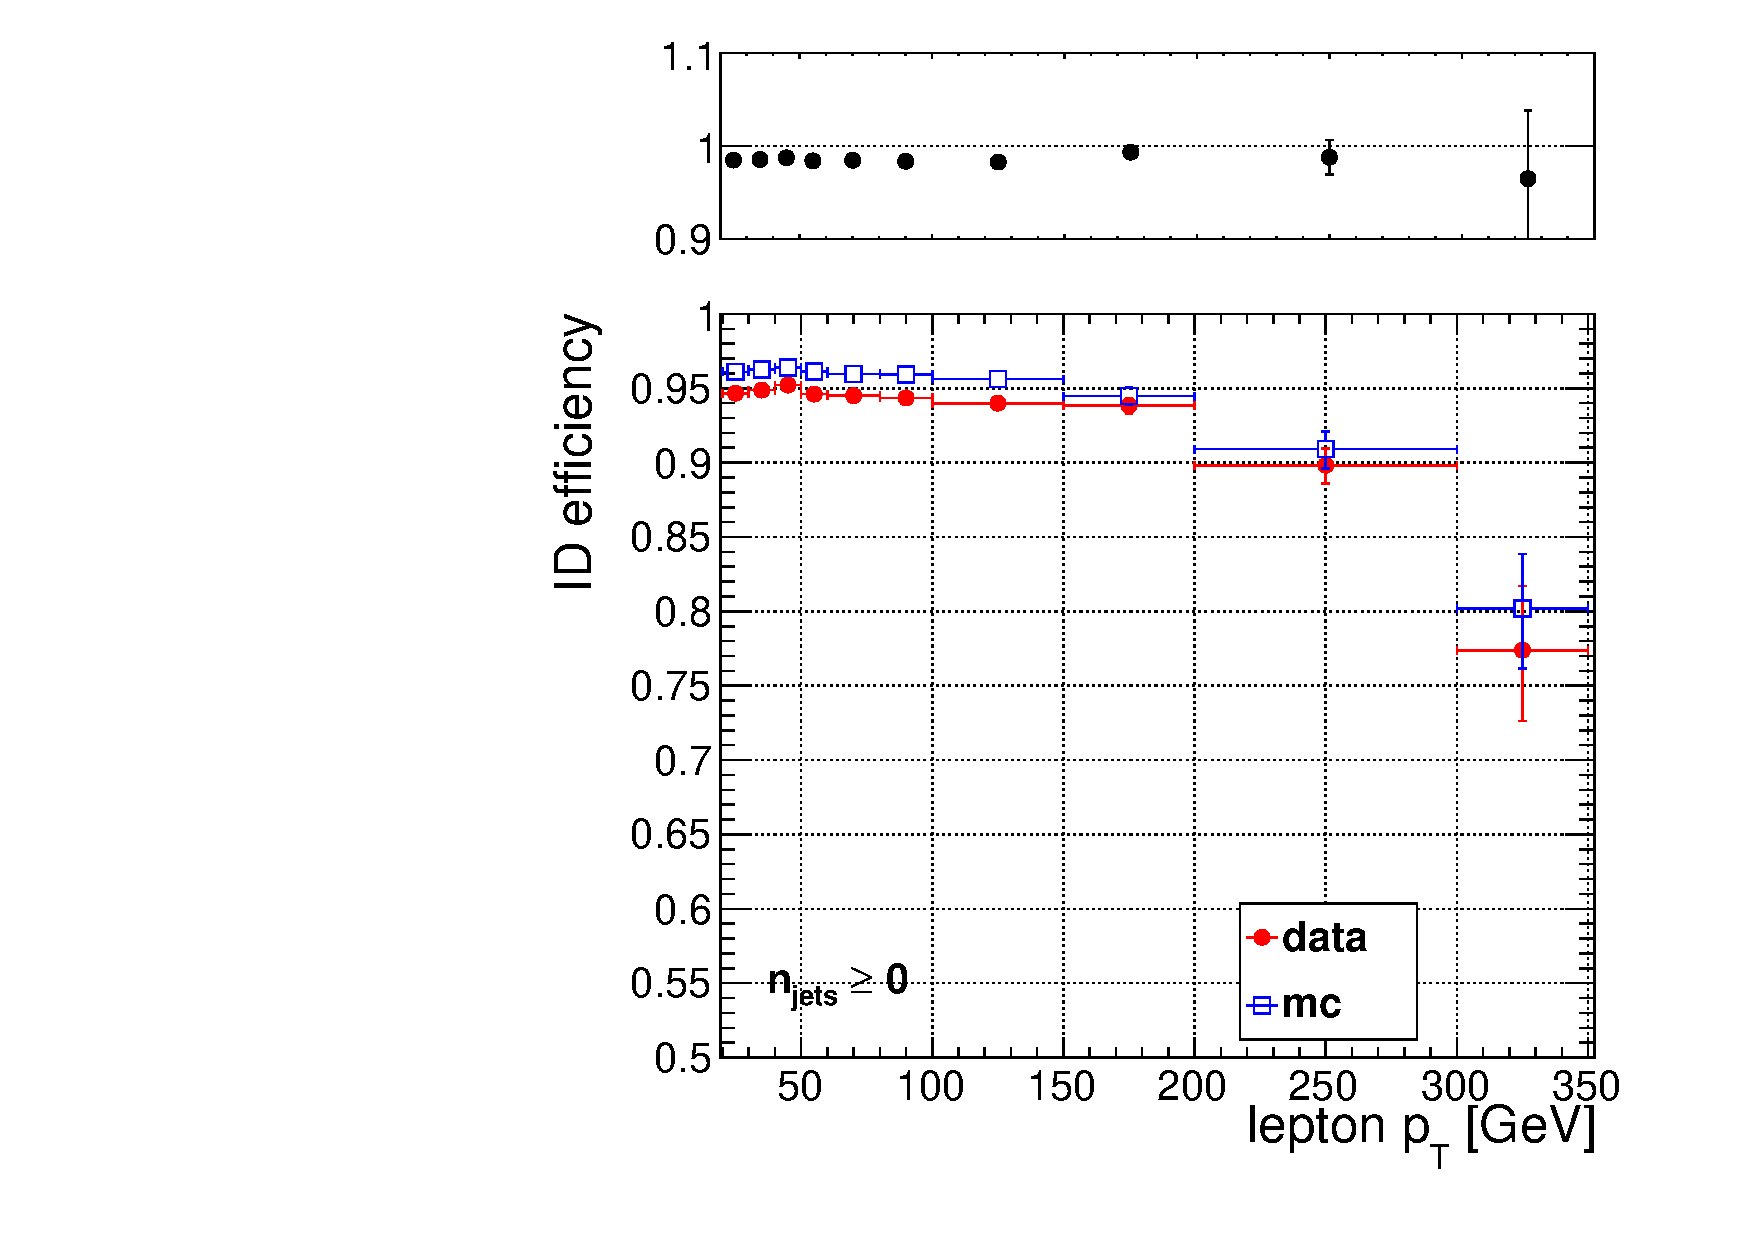
\includegraphics[width=0.3\linewidth]{plots/mu_id_njets0.pdf}%
	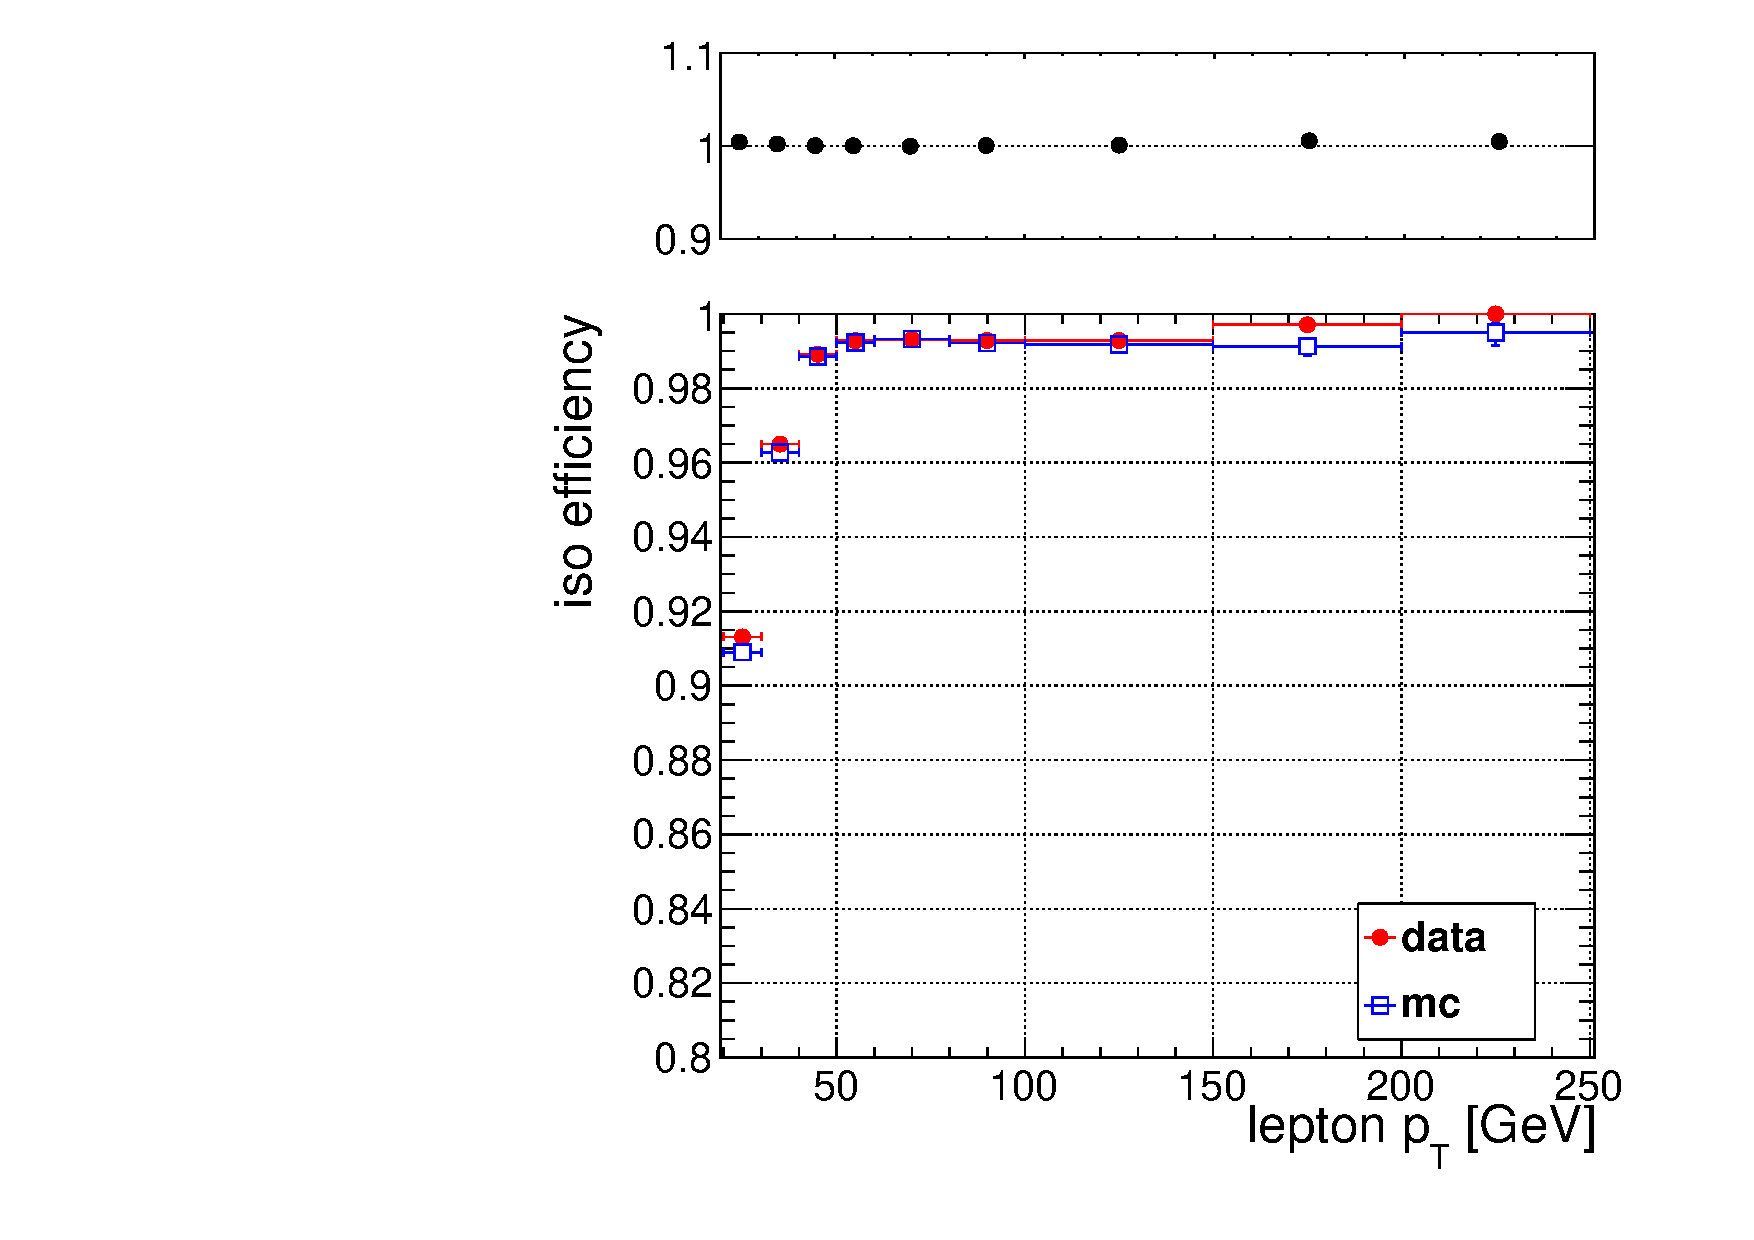
\includegraphics[width=0.3\linewidth]{plots/mu_iso_njets0.pdf}
	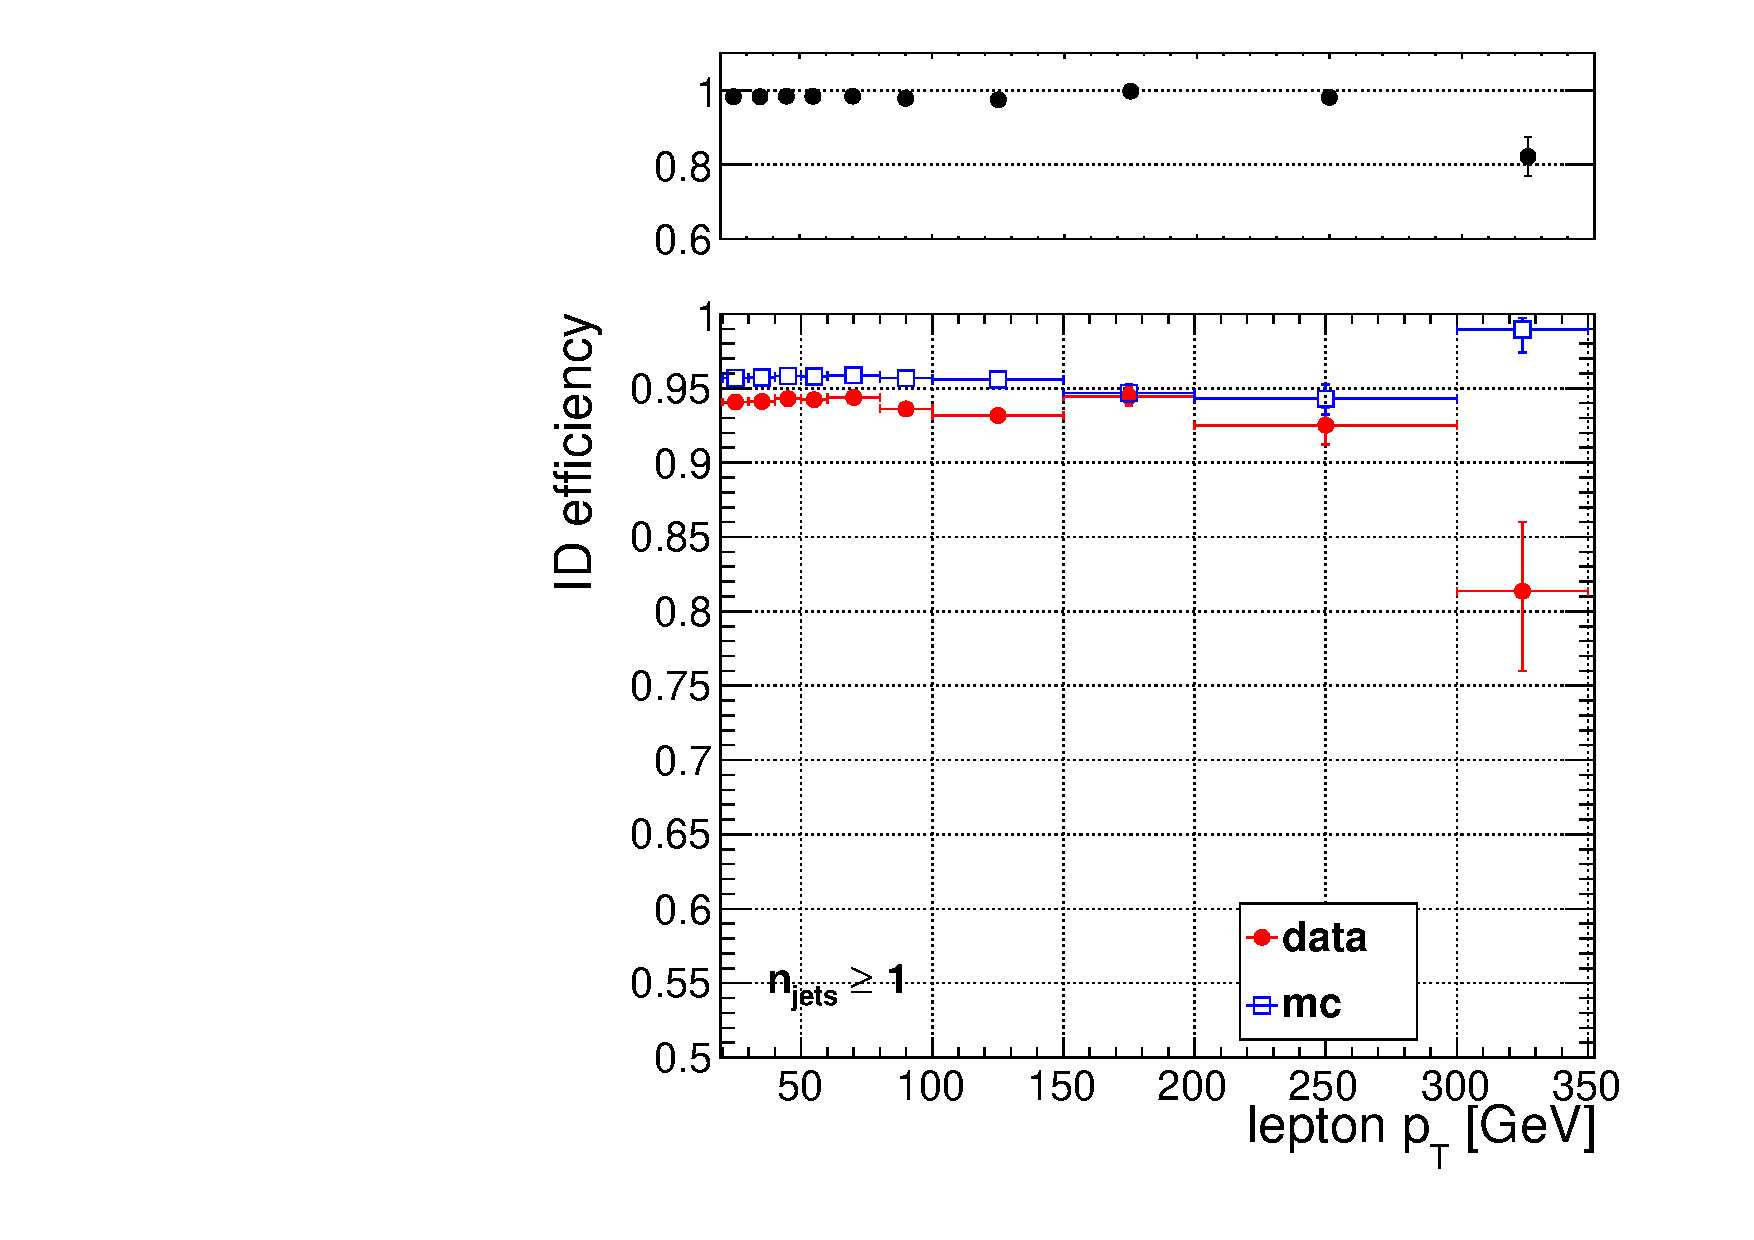
\includegraphics[width=0.3\linewidth]{plots/mu_id_njets1.pdf}%
	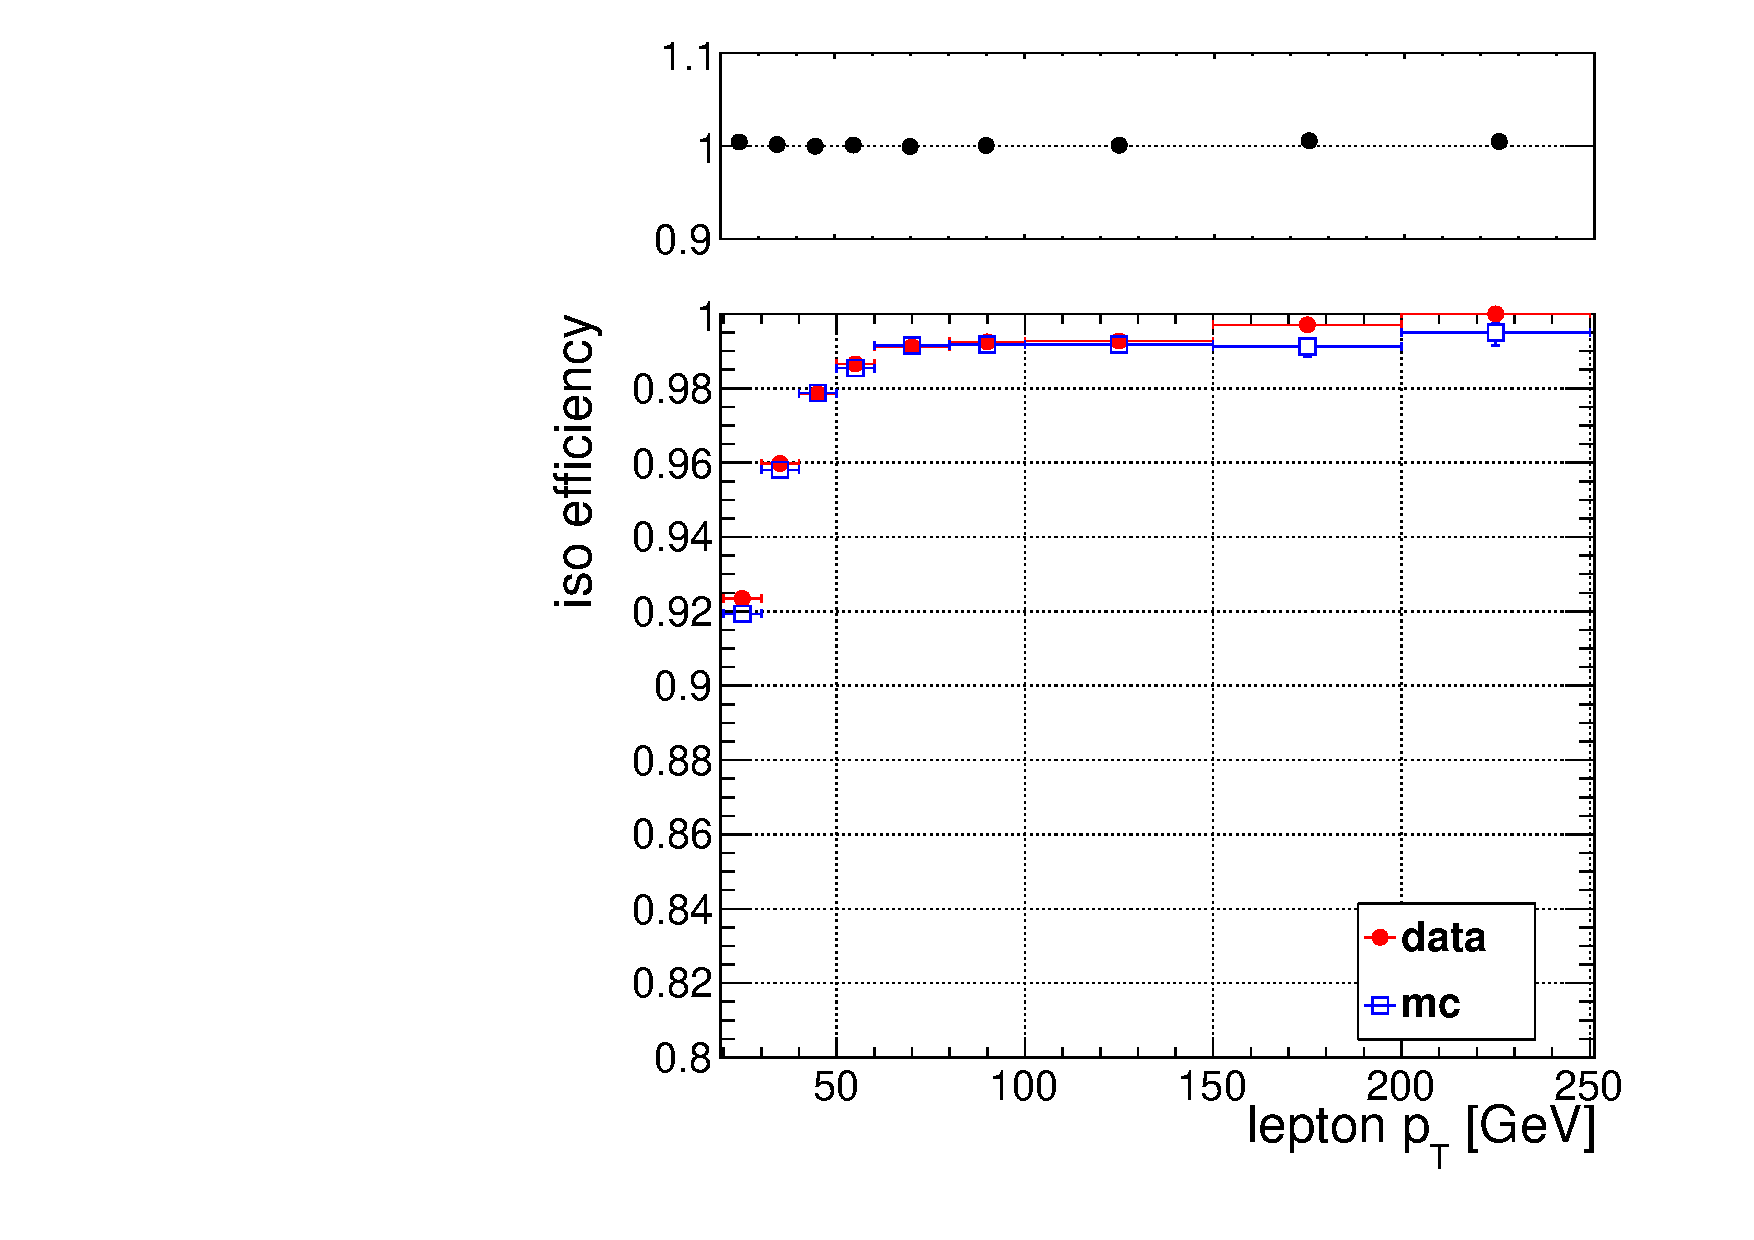
\includegraphics[width=0.3\linewidth]{plots/mu_iso_njets1.pdf}
	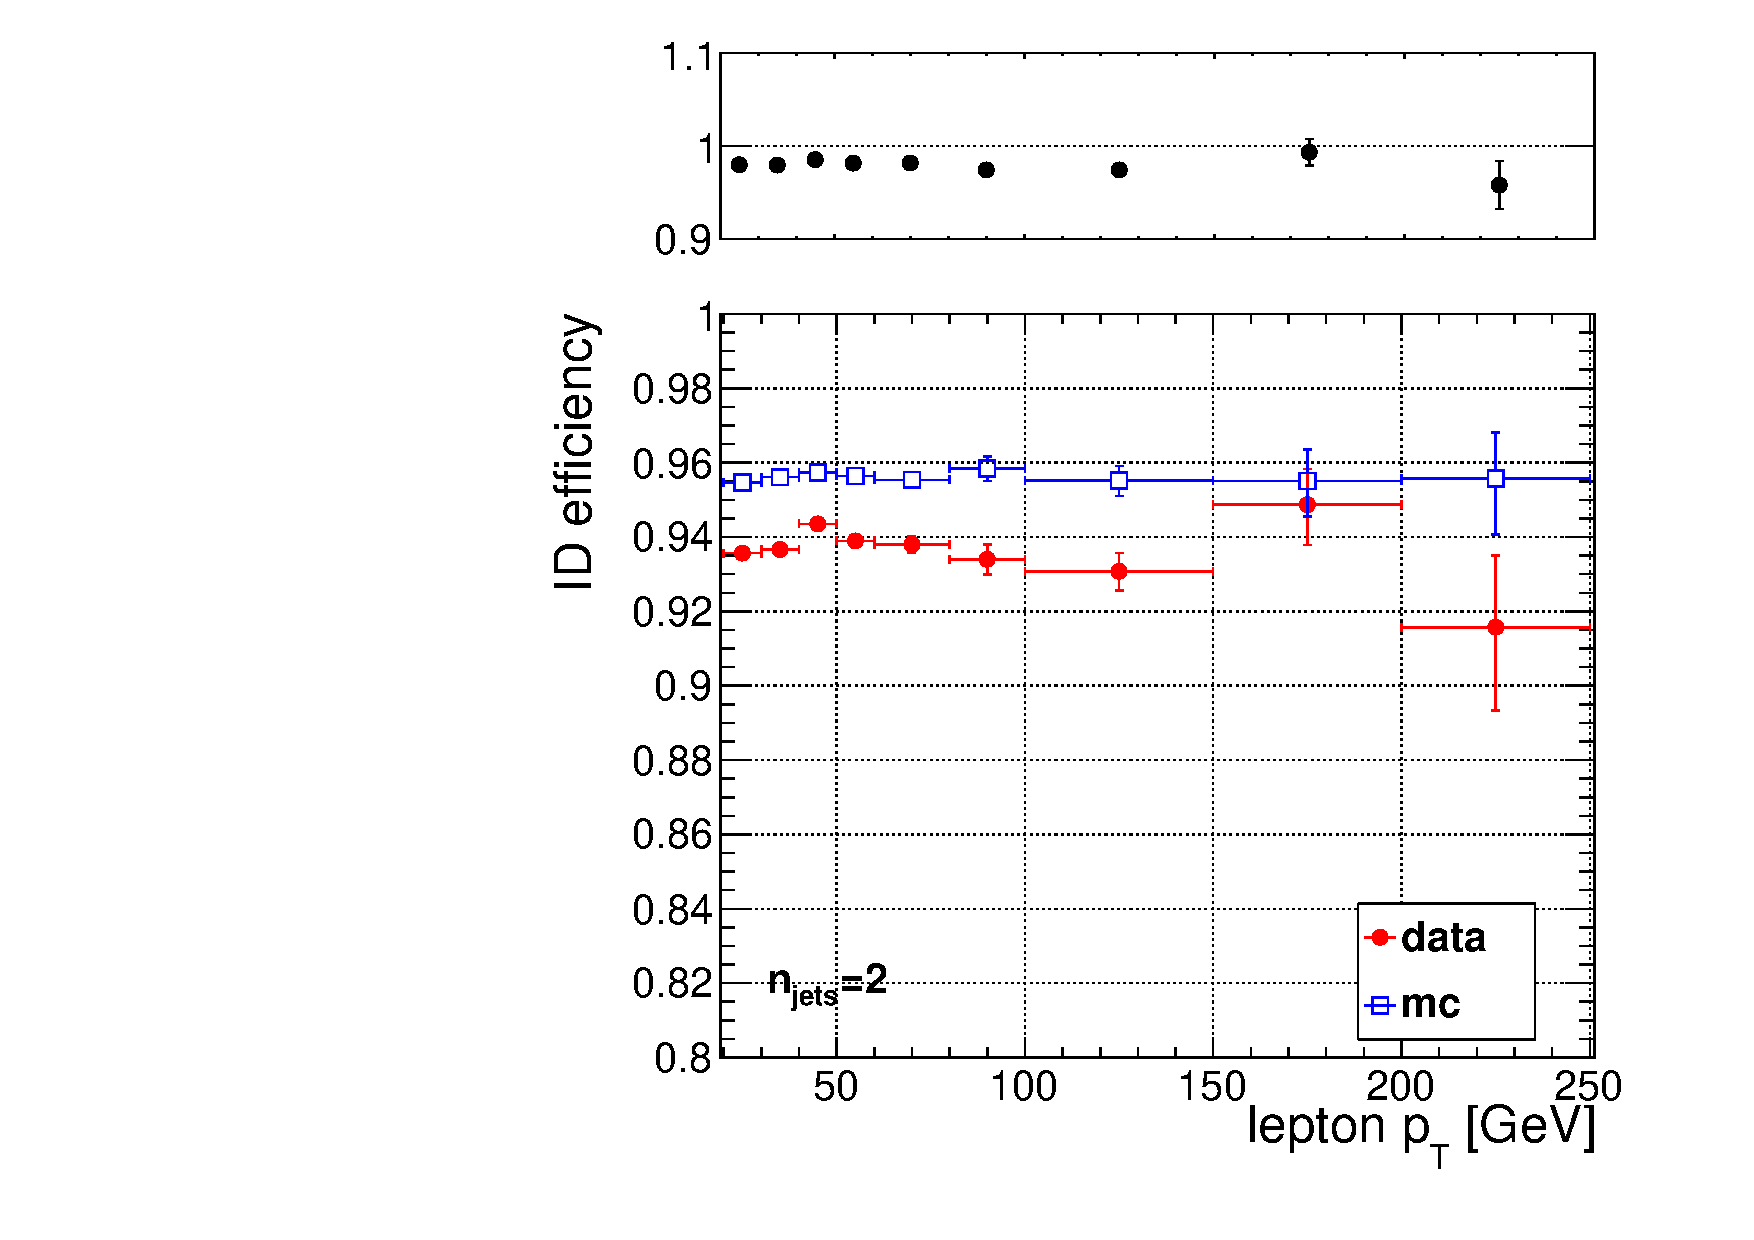
\includegraphics[width=0.3\linewidth]{plots/mu_id_njets2.pdf}%
	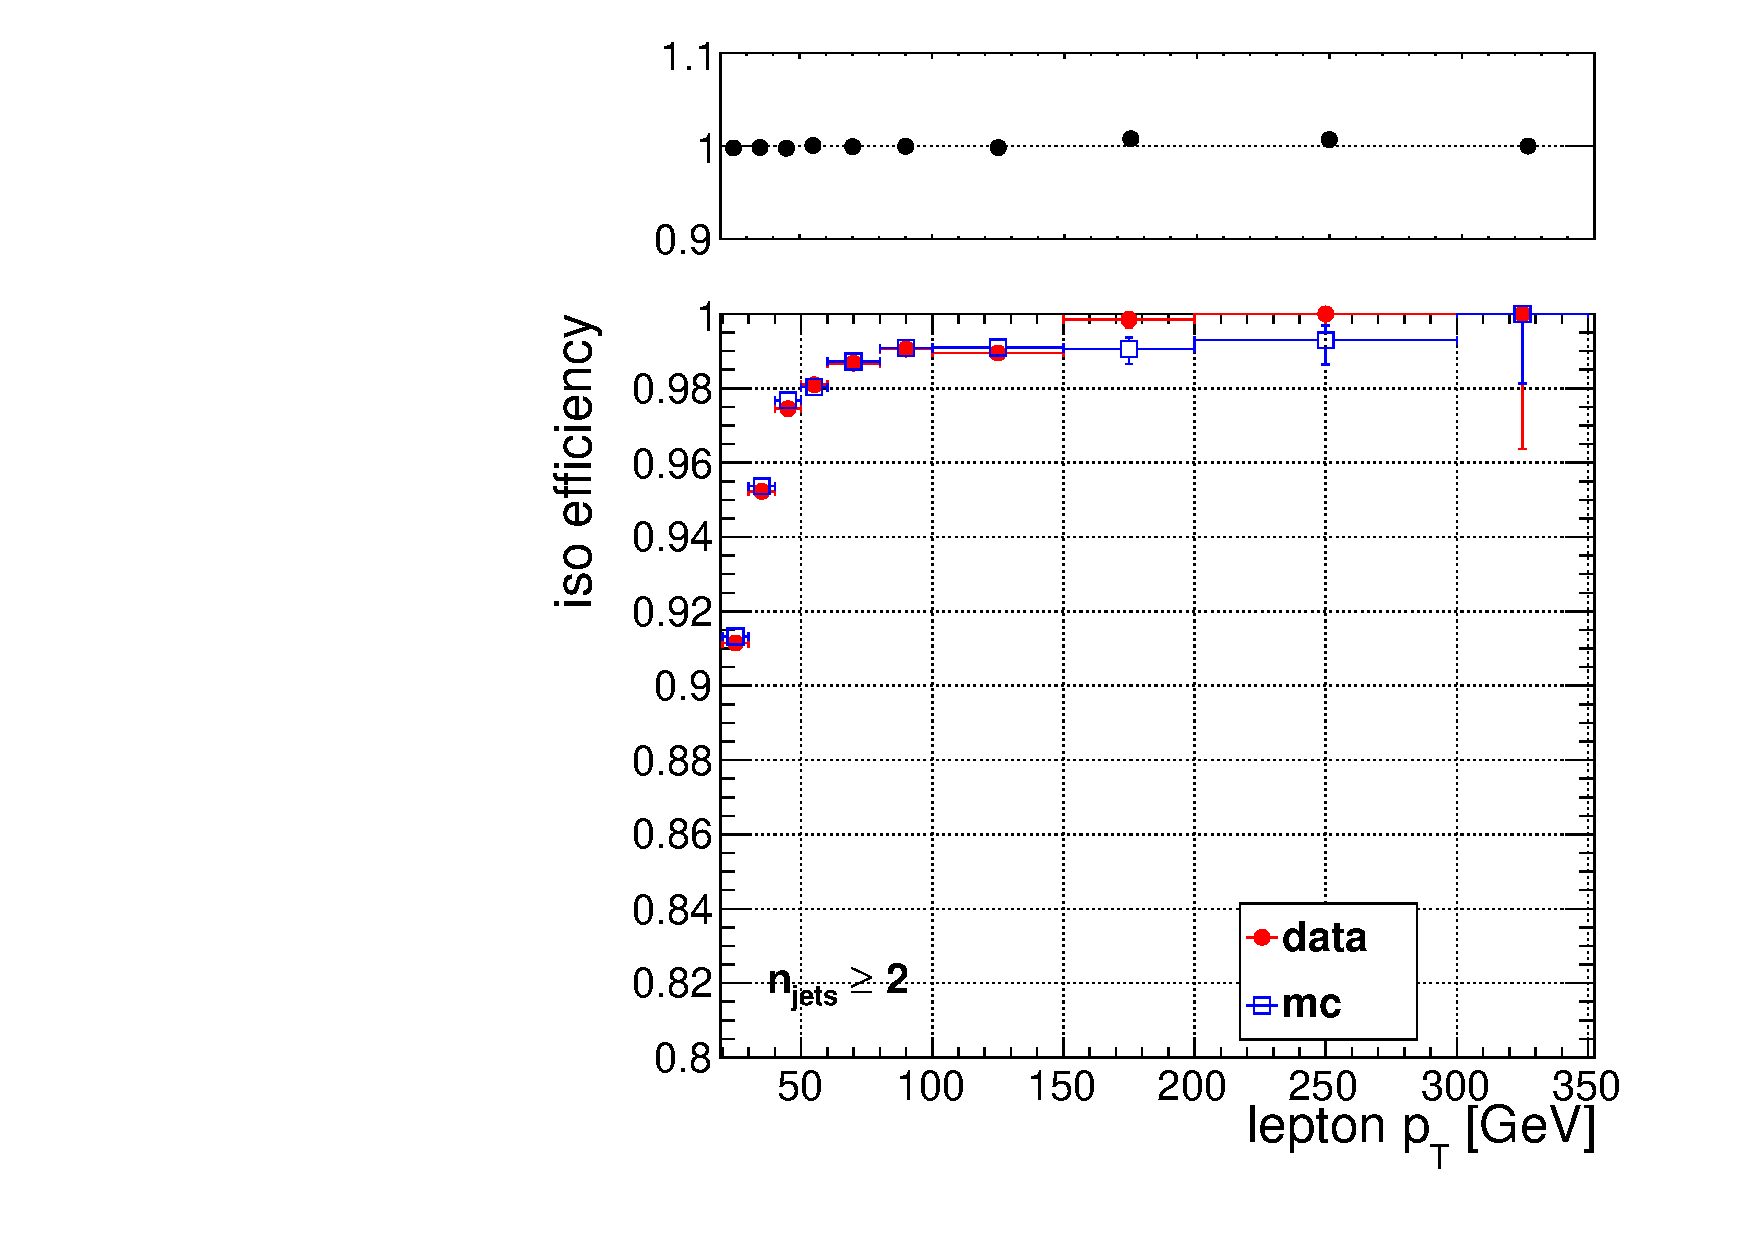
\includegraphics[width=0.3\linewidth]{plots/mu_iso_njets2.pdf}
	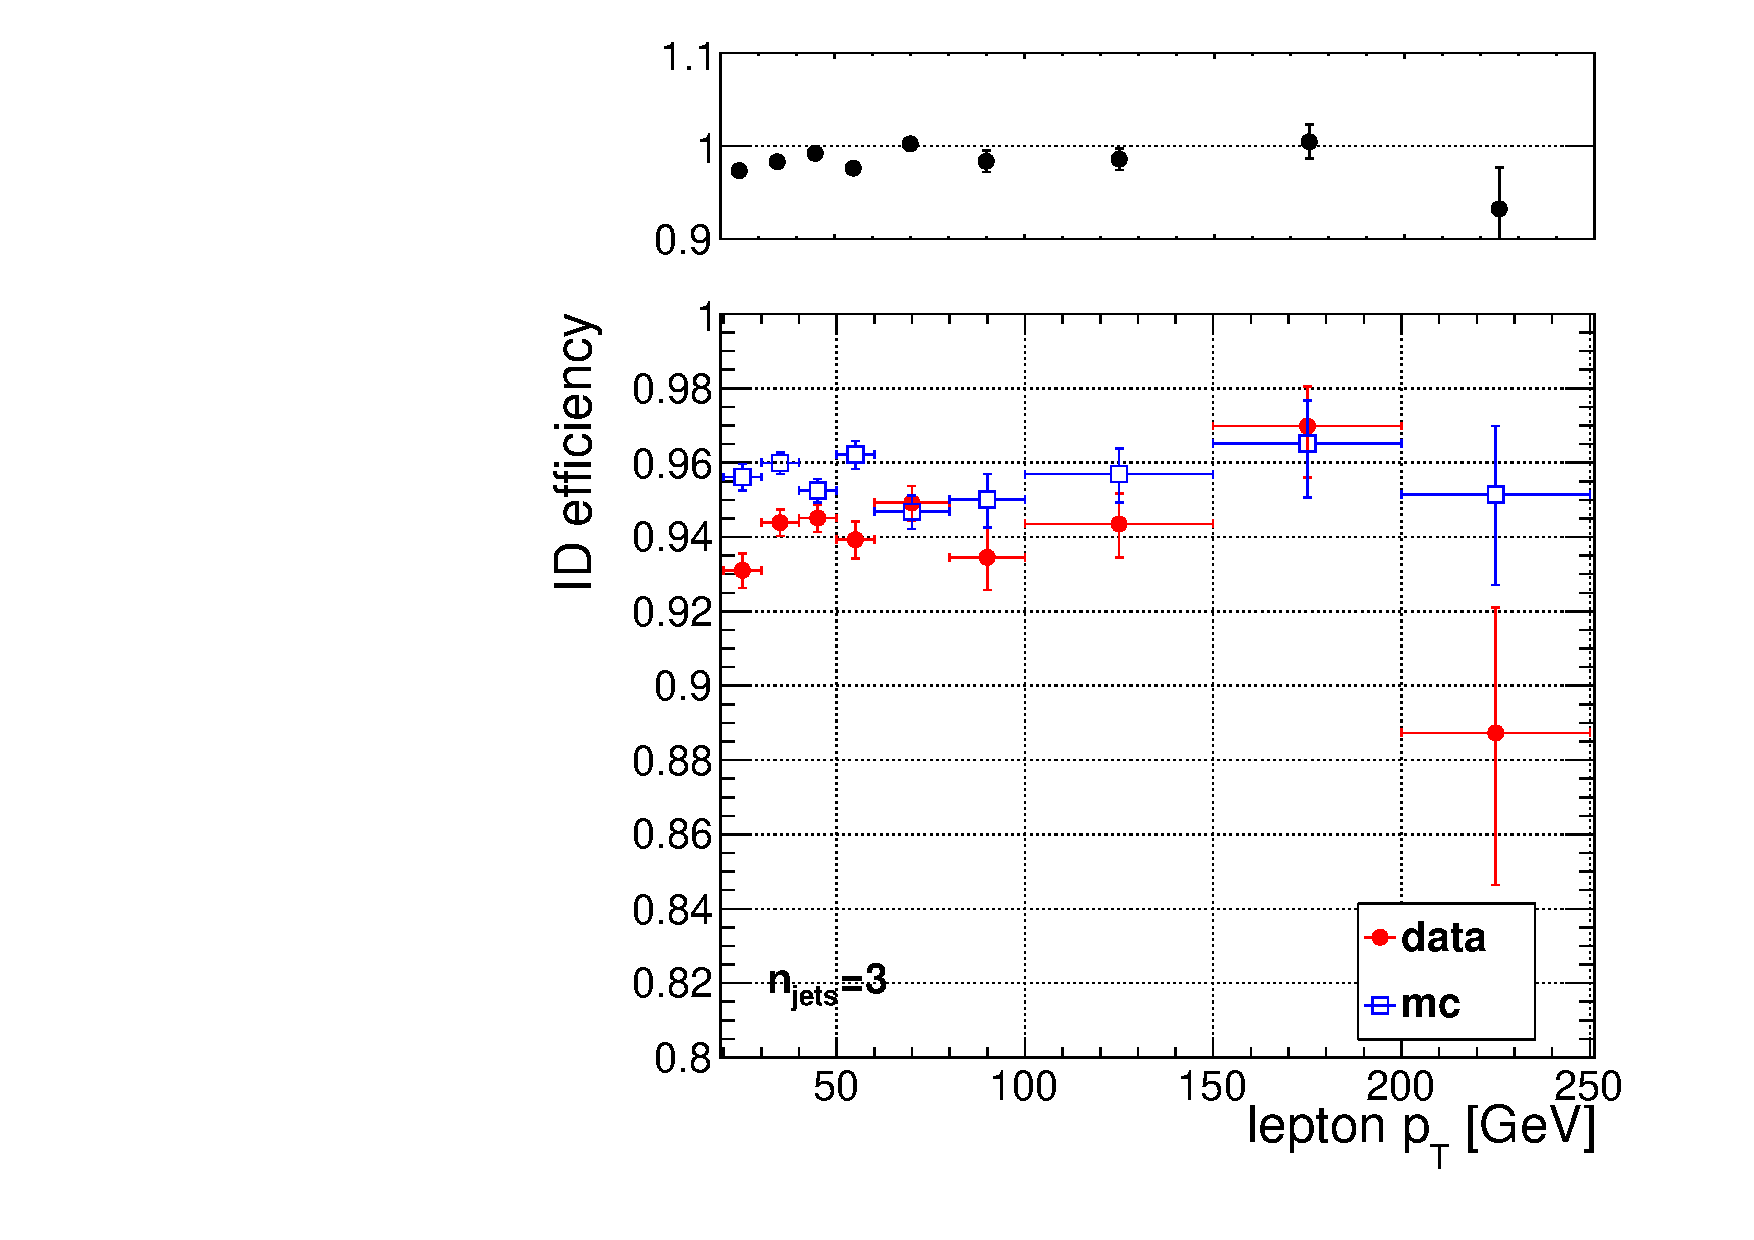
\includegraphics[width=0.3\linewidth]{plots/mu_id_njets3.pdf}%
	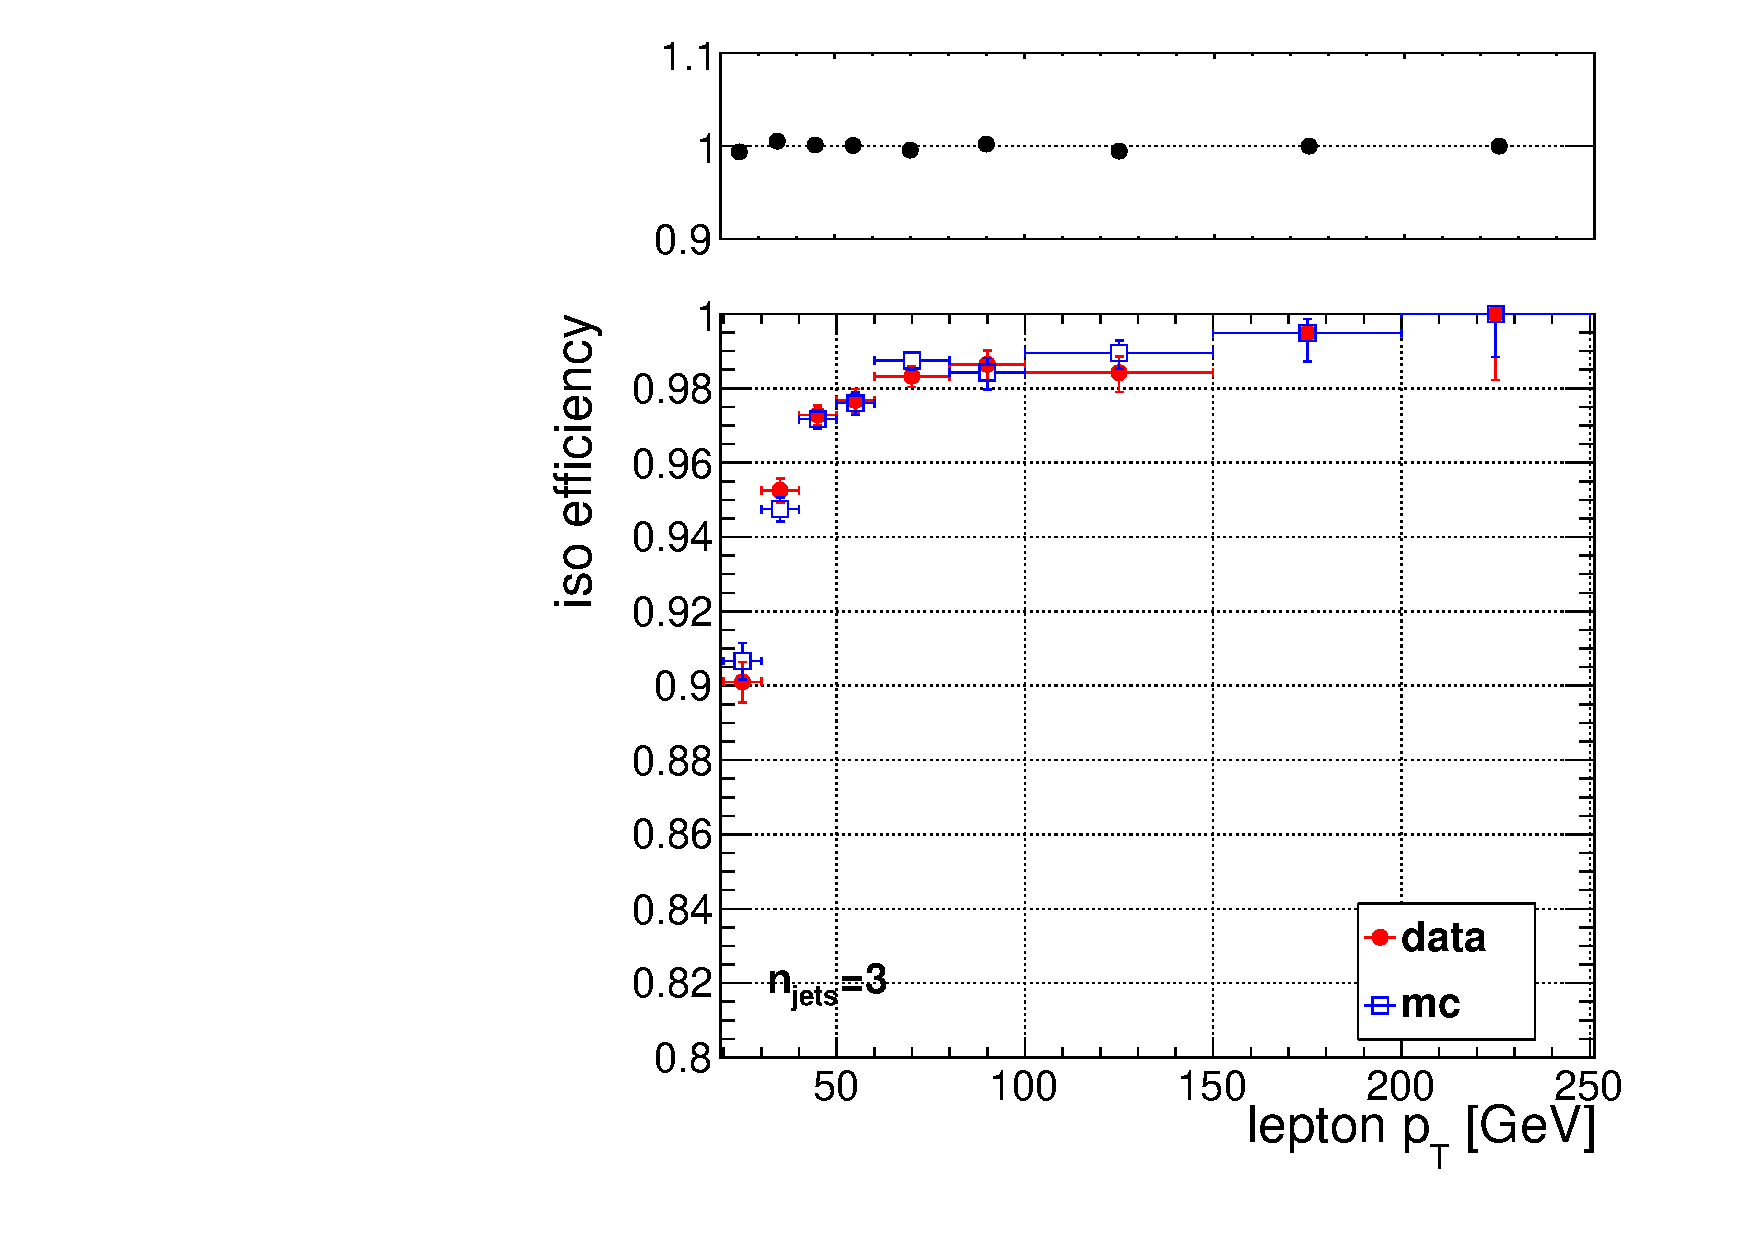
\includegraphics[width=0.3\linewidth]{plots/mu_iso_njets3.pdf}
	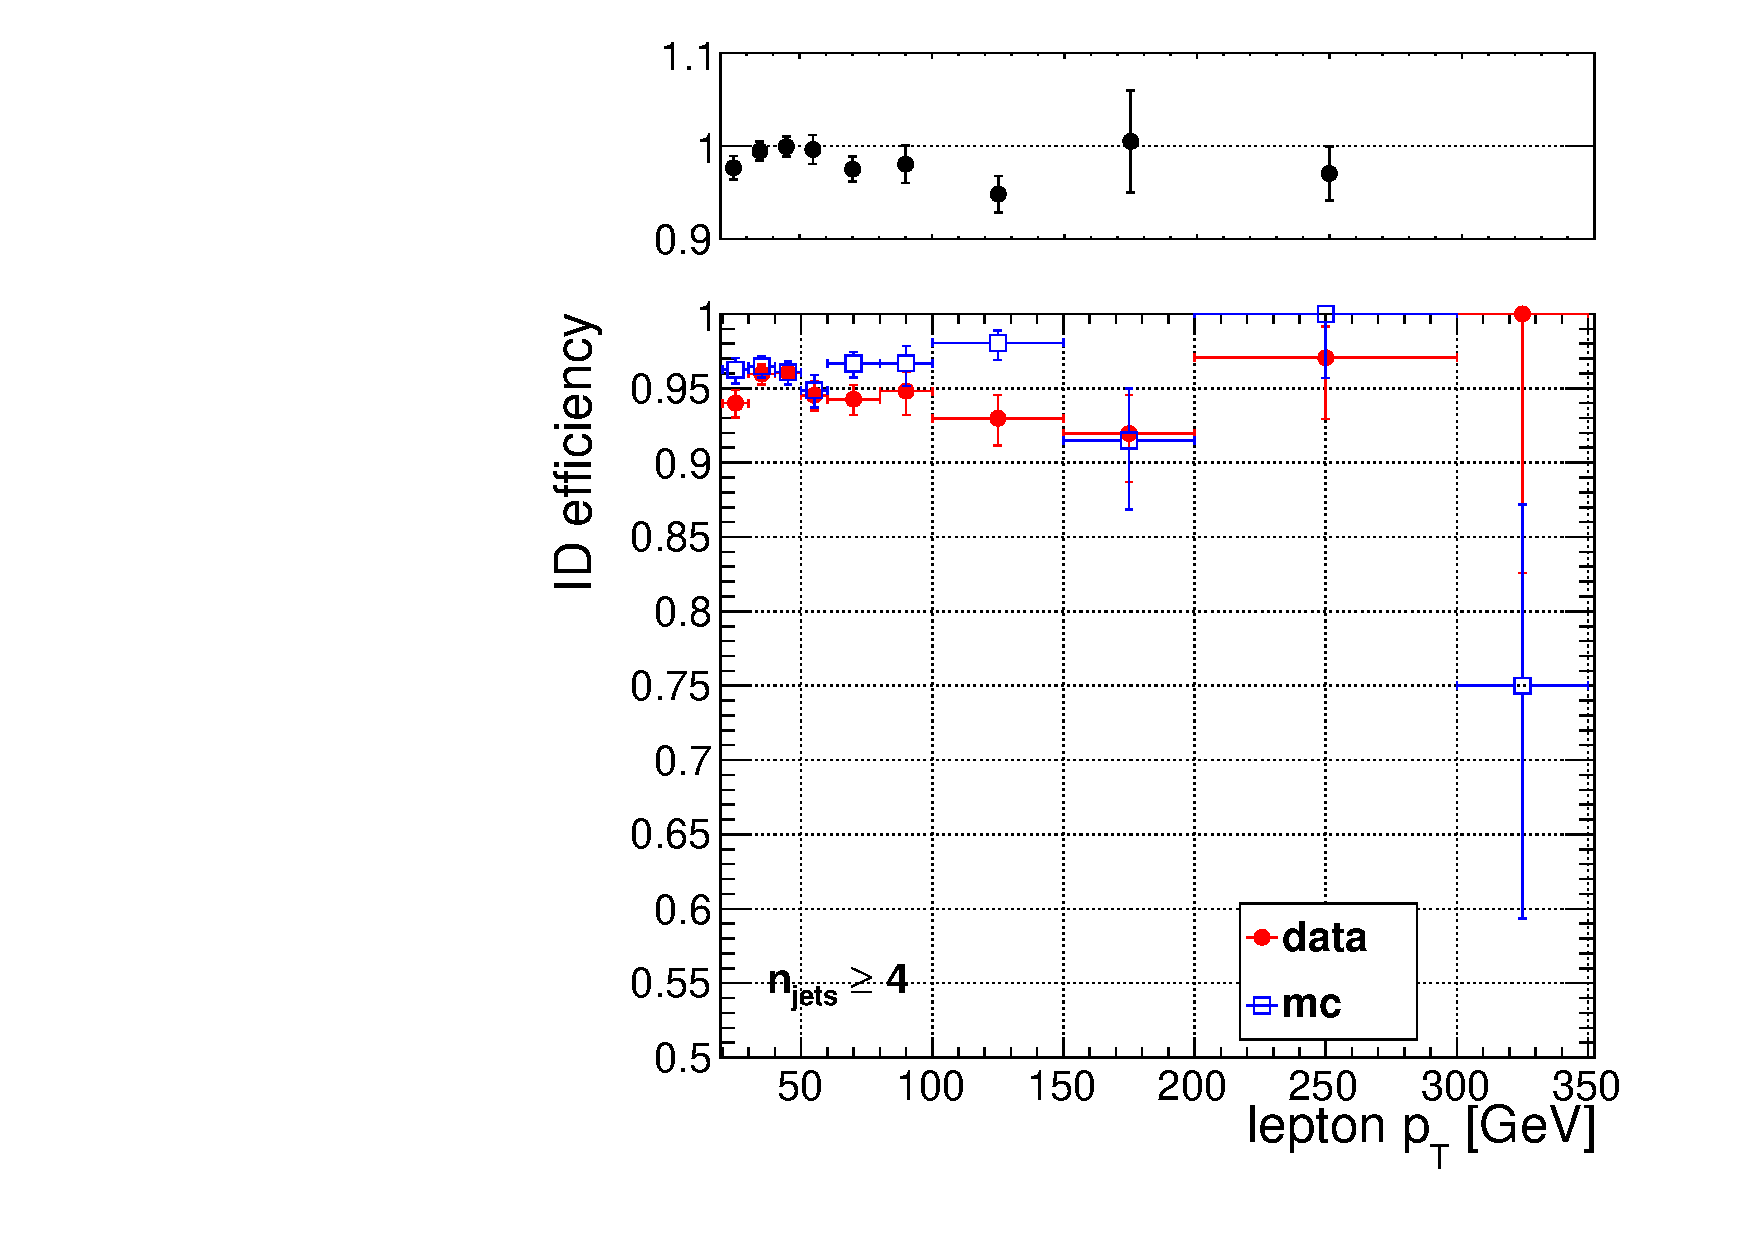
\includegraphics[width=0.3\linewidth]{plots/mu_id_njets4.pdf}%
	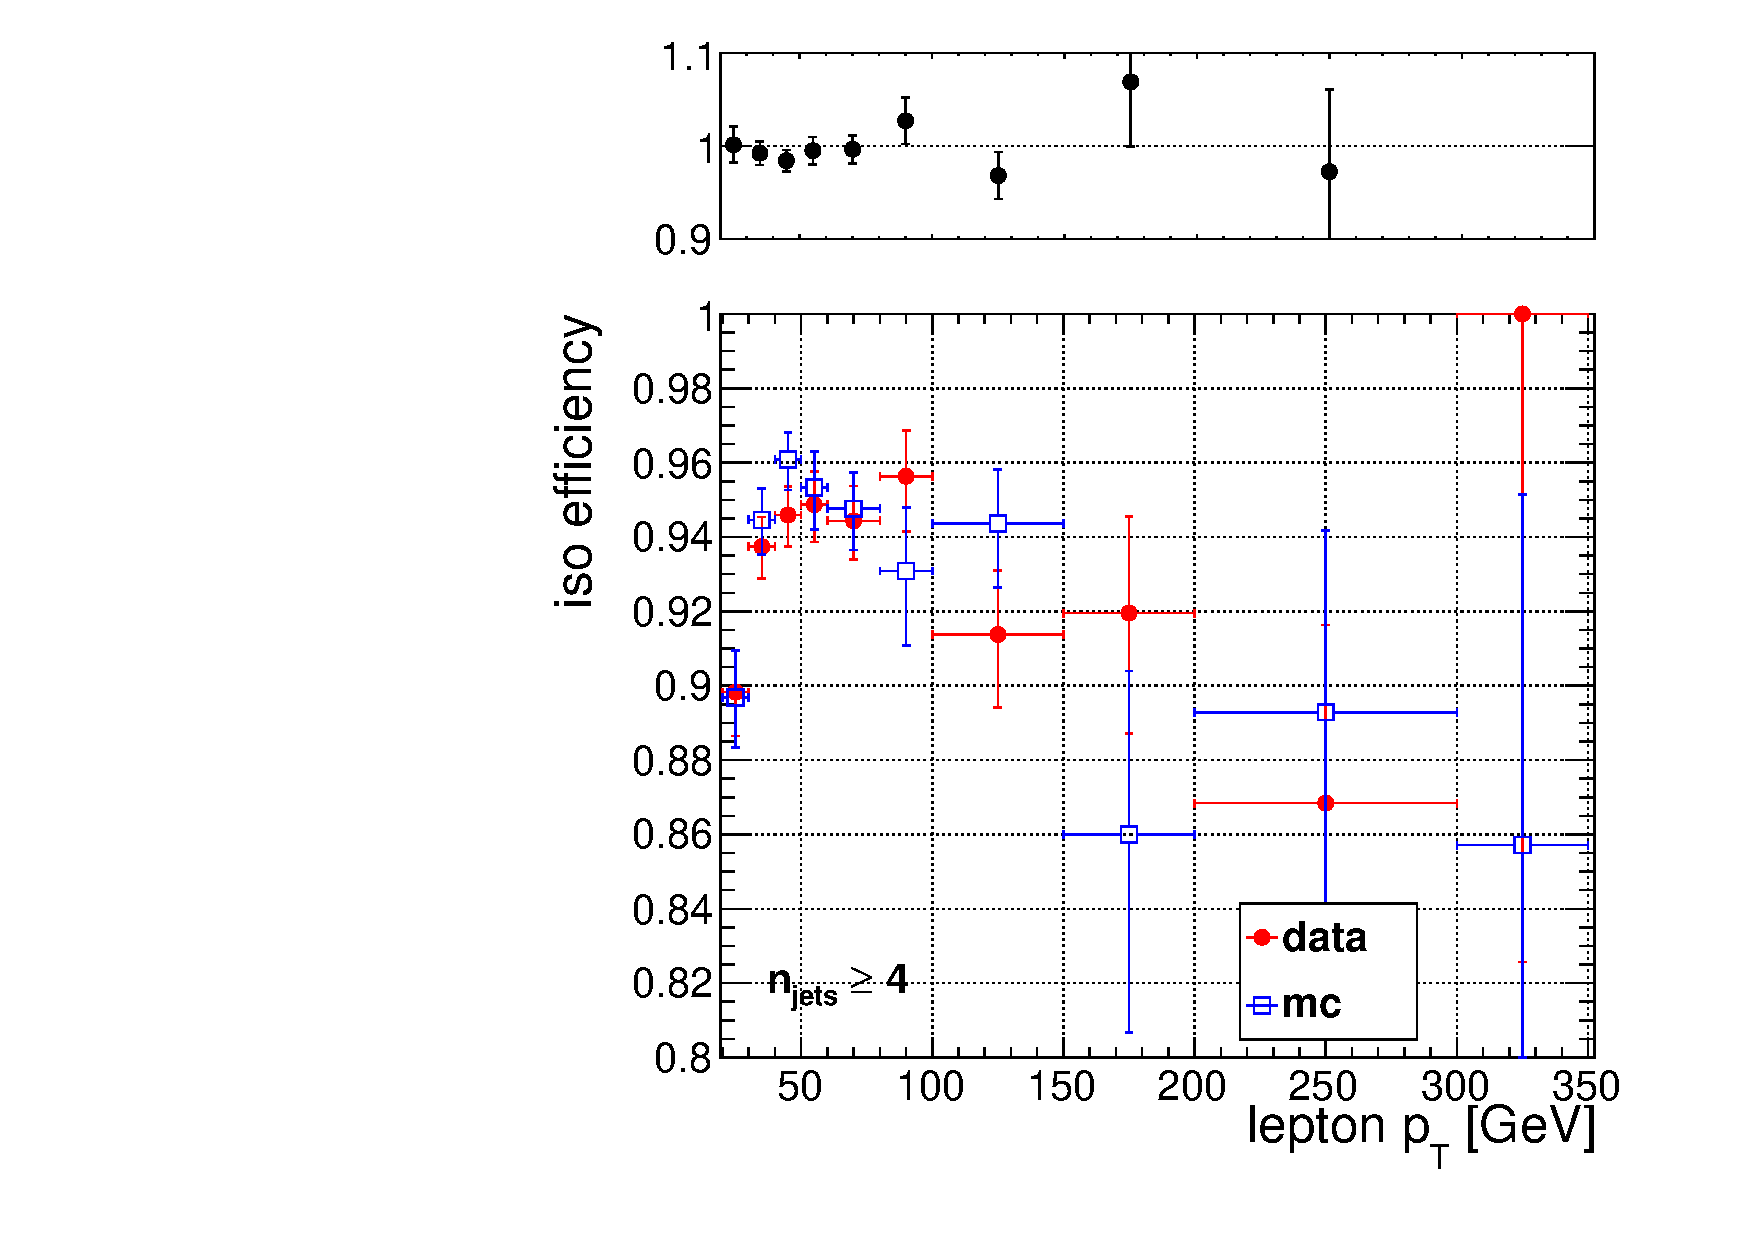
\includegraphics[width=0.3\linewidth]{plots/mu_iso_njets4.pdf}
	\caption{
	  \label{fig:mutnpeff} Comparison of the muon identification and isolation efficiencies in data and MC for various jet multiplicity requirements. }  
      \end{center}
\end{figure}

\clearpage

\begin{table}[htb]
\begin{center}
\scriptsize
\caption{\label{tab:eltnpeff}
Summary of the data and MC electron identification and isolation efficiencies measured with tag-and-probe studies.}
\begin{tabular}{c|c|c}

%Selection  : ((((((((abs(tagAndProbeMass-91)<15)&&(qProbe*qTag<0))&&(abs(tag->eta())<2.1))&&(tag->pt()>30.0))&&(abs(probe->eta())<2.1))&&(met<30))&&(nbl==0))&&((eventSelection&1)==1))&&(HLT_Ele27_WP80_tag > 0)
%Ndata      : 3577620
%NMC        : 3240624
%ID cut     : (leptonSelection&8)==8
%iso cut    : (leptonSelection&16)==16

\hline
\hline
MC ID & & \\
\pt\ range [GeV] & $|\eta|<1.5$ & $1.5<|\eta|<2.1$ \\
\hline
    20 -   30  & 	0.8156 $\pm$ 0.0008 & 	0.6565 $\pm$ 0.0019 \\
    30 -   40  & 	0.8670 $\pm$ 0.0004 & 	0.7450 $\pm$ 0.0010 \\
    40 -   50  & 	0.8922 $\pm$ 0.0003 & 	0.7847 $\pm$ 0.0008 \\
    50 -   60  & 	0.9023 $\pm$ 0.0006 & 	0.7956 $\pm$ 0.0018 \\
    60 -   80  & 	0.9097 $\pm$ 0.0011 & 	0.8166 $\pm$ 0.0034 \\
    80 -  100  & 	0.9203 $\pm$ 0.0028 & 	0.8196 $\pm$ 0.0090 \\
   100 -  150  & 	0.9162 $\pm$ 0.0037 & 	0.8378 $\pm$ 0.0117 \\
   150 -  200  & 	0.9106 $\pm$ 0.0087 & 	0.8111 $\pm$ 0.0292 \\
   200 -  300  & 	0.9304 $\pm$ 0.0119 & 	0.9153 $\pm$ 0.0363 \\
   300 - 10000  & 	0.8684 $\pm$ 0.0388 & 	0.8000 $\pm$ 0.1789 \\
\hline
\hline
MC ISO  & & \\

\pt\ range [GeV] & $|\eta|<1.5$ & $1.5<|\eta|<2.1$ \\
\hline
    20 -   30  & 	0.9245 $\pm$ 0.0006 & 	0.9466 $\pm$ 0.0011 \\
    30 -   40  & 	0.9682 $\pm$ 0.0002 & 	0.9741 $\pm$ 0.0004 \\
    40 -   50  & 	0.9876 $\pm$ 0.0001 & 	0.9883 $\pm$ 0.0002 \\
    50 -   60  & 	0.9909 $\pm$ 0.0002 & 	0.9912 $\pm$ 0.0005 \\
    60 -   80  & 	0.9916 $\pm$ 0.0004 & 	0.9930 $\pm$ 0.0008 \\
    80 -  100  & 	0.9915 $\pm$ 0.0010 & 	0.9908 $\pm$ 0.0025 \\
   100 -  150  & 	0.9929 $\pm$ 0.0012 & 	0.9894 $\pm$ 0.0035 \\
   150 -  200  & 	0.9919 $\pm$ 0.0029 & 	0.9932 $\pm$ 0.0068 \\
   200 -  300  & 	0.9953 $\pm$ 0.0033 & 	1.0000 $\pm$ 0.0000 \\
   300 - 10000  & 	1.0000 $\pm$ 0.0000 & 	1.0000 $\pm$ 0.0000 \\
\hline
\hline
DATA ID & & \\

\pt\ range [GeV] & $|\eta|<1.5$ & $1.5<|\eta|<2.1$ \\
\hline
    20 -   30  & 	0.8145 $\pm$ 0.0008 & 	0.6528 $\pm$ 0.0018 \\
    30 -   40  & 	0.8676 $\pm$ 0.0004 & 	0.7462 $\pm$ 0.0010 \\
    40 -   50  & 	0.8955 $\pm$ 0.0003 & 	0.7922 $\pm$ 0.0008 \\
    50 -   60  & 	0.9049 $\pm$ 0.0006 & 	0.8072 $\pm$ 0.0018 \\
    60 -   80  & 	0.9110 $\pm$ 0.0011 & 	0.8212 $\pm$ 0.0035 \\
    80 -  100  & 	0.9156 $\pm$ 0.0028 & 	0.8358 $\pm$ 0.0091 \\
   100 -  150  & 	0.9257 $\pm$ 0.0036 & 	0.8507 $\pm$ 0.0116 \\
   150 -  200  & 	0.9186 $\pm$ 0.0084 & 	0.8929 $\pm$ 0.0292 \\
   200 -  300  & 	0.9106 $\pm$ 0.0149 & 	0.7576 $\pm$ 0.0746 \\
   300 - 10000  & 	0.9400 $\pm$ 0.0336 & 	1.0000 $\pm$ 0.0000 \\
\hline
\hline
DATA ISO  & & \\

\pt\ range [GeV] & $|\eta|<1.5$ & $1.5<|\eta|<2.1$ \\
\hline
    20 -   30  & 	0.9201 $\pm$ 0.0006 & 	0.9419 $\pm$ 0.0011 \\
    30 -   40  & 	0.9667 $\pm$ 0.0002 & 	0.9734 $\pm$ 0.0004 \\
    40 -   50  & 	0.9872 $\pm$ 0.0001 & 	0.9892 $\pm$ 0.0002 \\
    50 -   60  & 	0.9904 $\pm$ 0.0002 & 	0.9922 $\pm$ 0.0004 \\
    60 -   80  & 	0.9923 $\pm$ 0.0004 & 	0.9916 $\pm$ 0.0009 \\
    80 -  100  & 	0.9914 $\pm$ 0.0010 & 	0.9921 $\pm$ 0.0024 \\
   100 -  150  & 	0.9945 $\pm$ 0.0011 & 	1.0000 $\pm$ 0.0000 \\
   150 -  200  & 	0.9908 $\pm$ 0.0031 & 	1.0000 $\pm$ 0.0000 \\
   200 -  300  & 	0.9941 $\pm$ 0.0042 & 	1.0000 $\pm$ 0.0000 \\
   300 - 10000  & 	0.9792 $\pm$ 0.0206 & 	1.0000 $\pm$ 0.0000 \\
\hline
\hline
 Scale Factor ID  & & \\

\pt\ range [GeV] & $|\eta|<1.5$ & $1.5<|\eta|<2.1$ \\
\hline
    20 -   30  & 	0.9987 $\pm$ 0.0014 & 	0.9944 $\pm$ 0.0040 \\
    30 -   40  & 	1.0007 $\pm$ 0.0006 & 	1.0015 $\pm$ 0.0019 \\
    40 -   50  & 	1.0036 $\pm$ 0.0005 & 	1.0096 $\pm$ 0.0015 \\
    50 -   60  & 	1.0029 $\pm$ 0.0010 & 	1.0146 $\pm$ 0.0031 \\
    60 -   80  & 	1.0014 $\pm$ 0.0018 & 	1.0057 $\pm$ 0.0060 \\
    80 -  100  & 	0.9949 $\pm$ 0.0043 & 	1.0197 $\pm$ 0.0158 \\
   100 -  150  & 	1.0104 $\pm$ 0.0057 & 	1.0154 $\pm$ 0.0198 \\
   150 -  200  & 	1.0087 $\pm$ 0.0134 & 	1.1008 $\pm$ 0.0535 \\
   200 -  300  & 	0.9786 $\pm$ 0.0203 & 	0.8277 $\pm$ 0.0879 \\
   300 - 10000  & 	1.0824 $\pm$ 0.0619 & 	1.2500 $\pm$ 0.2795 \\
\hline
\hline
Scale Factor ISO & & \\
\pt\ range [GeV] & $|\eta|<1.5$ & $1.5<|\eta|<2.1$ \\
\hline
    20 -   30  & 	0.9952 $\pm$ 0.0009 & 	0.9950 $\pm$ 0.0016 \\
    30 -   40  & 	0.9984 $\pm$ 0.0003 & 	0.9992 $\pm$ 0.0006 \\
    40 -   50  & 	0.9996 $\pm$ 0.0002 & 	1.0009 $\pm$ 0.0003 \\
    50 -   60  & 	0.9995 $\pm$ 0.0003 & 	1.0009 $\pm$ 0.0006 \\
    60 -   80  & 	1.0006 $\pm$ 0.0005 & 	0.9985 $\pm$ 0.0012 \\
    80 -  100  & 	0.9999 $\pm$ 0.0014 & 	1.0013 $\pm$ 0.0035 \\
   100 -  150  & 	1.0016 $\pm$ 0.0016 & 	1.0108 $\pm$ 0.0036 \\
   150 -  200  & 	0.9989 $\pm$ 0.0042 & 	1.0068 $\pm$ 0.0069 \\
   200 -  300  & 	0.9987 $\pm$ 0.0053 & 	1.0000 $\pm$ 0.0000 \\
   300 - 10000  & 	0.9792 $\pm$ 0.0206 & 	1.0000 $\pm$ 0.0000 \\
\hline
\hline

\end{tabular}
\end{center}
\end{table}

\begin{figure}[hbt]
  \begin{center}
    	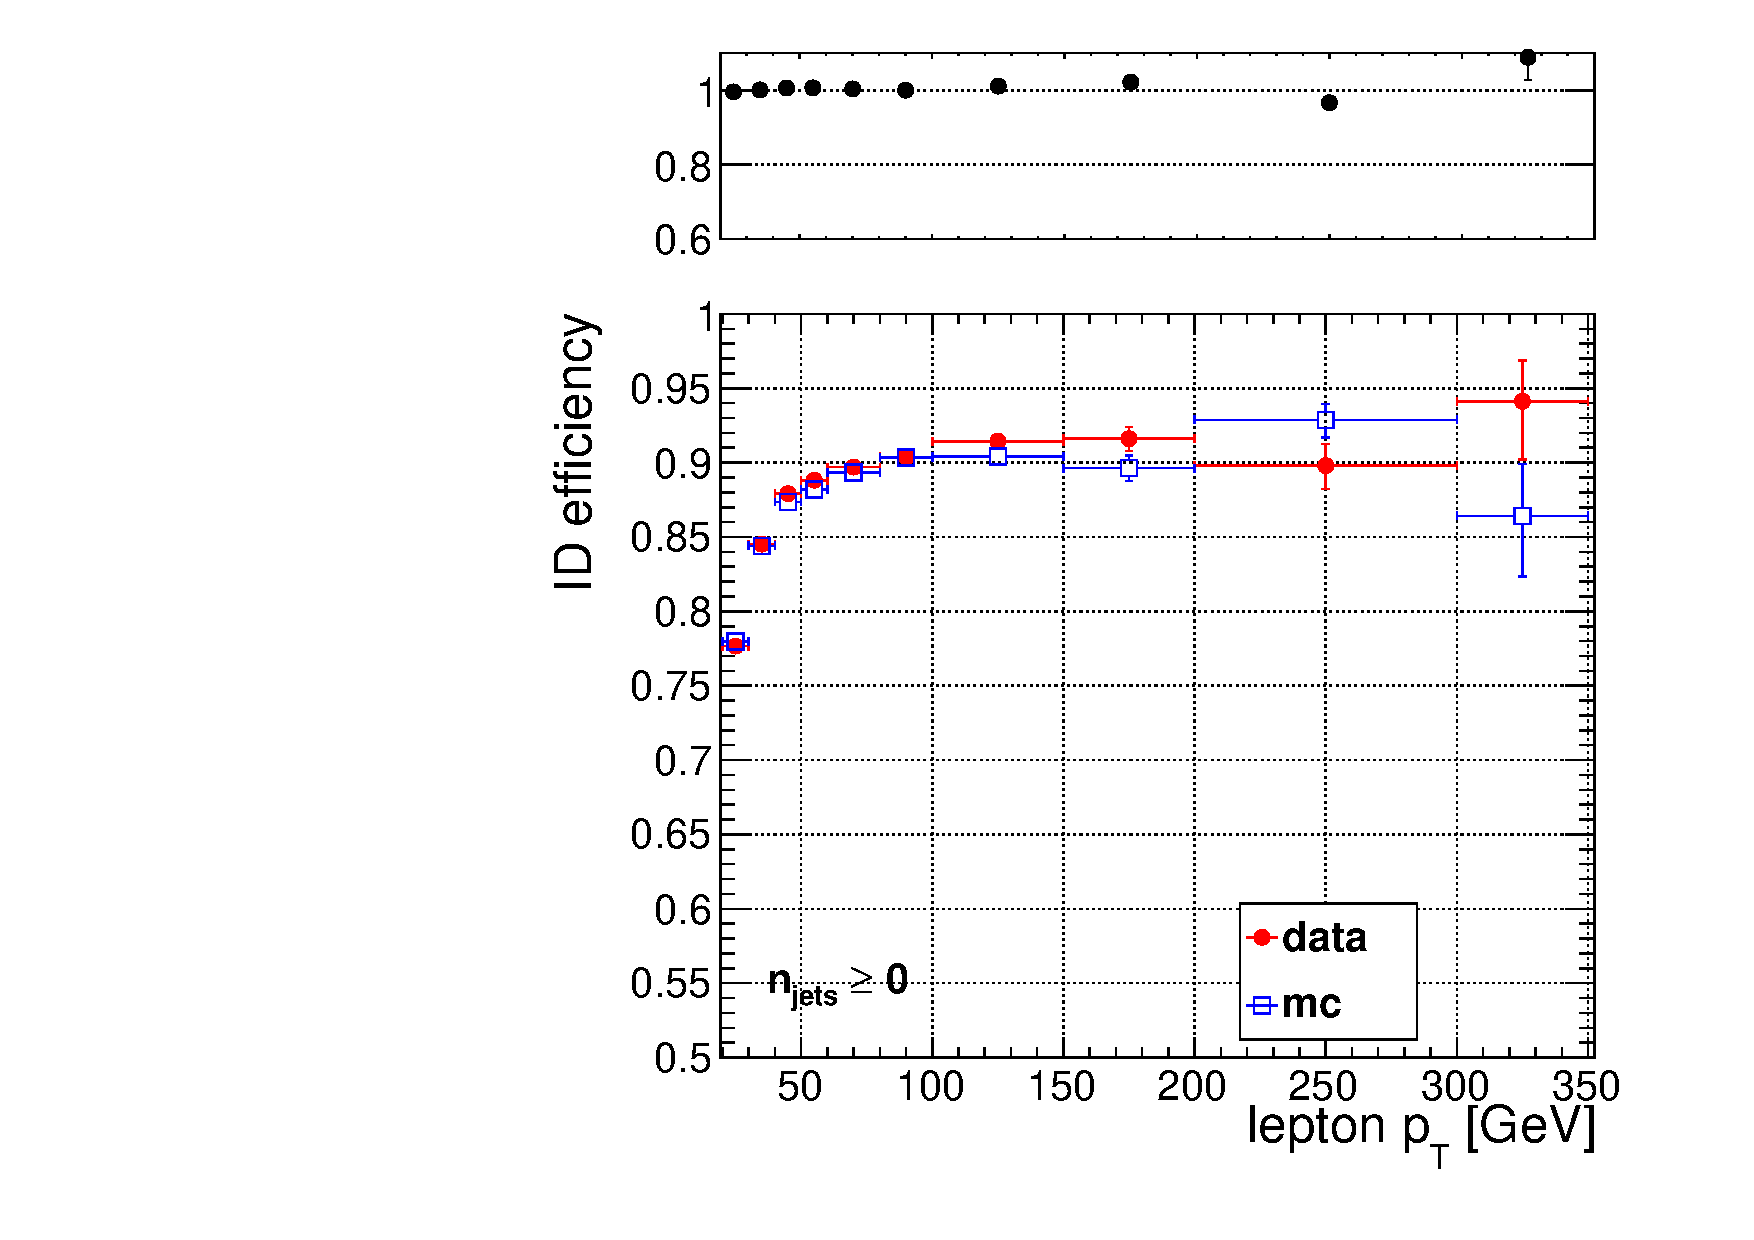
\includegraphics[width=0.3\linewidth]{plots/el_id_njets0.pdf}%
	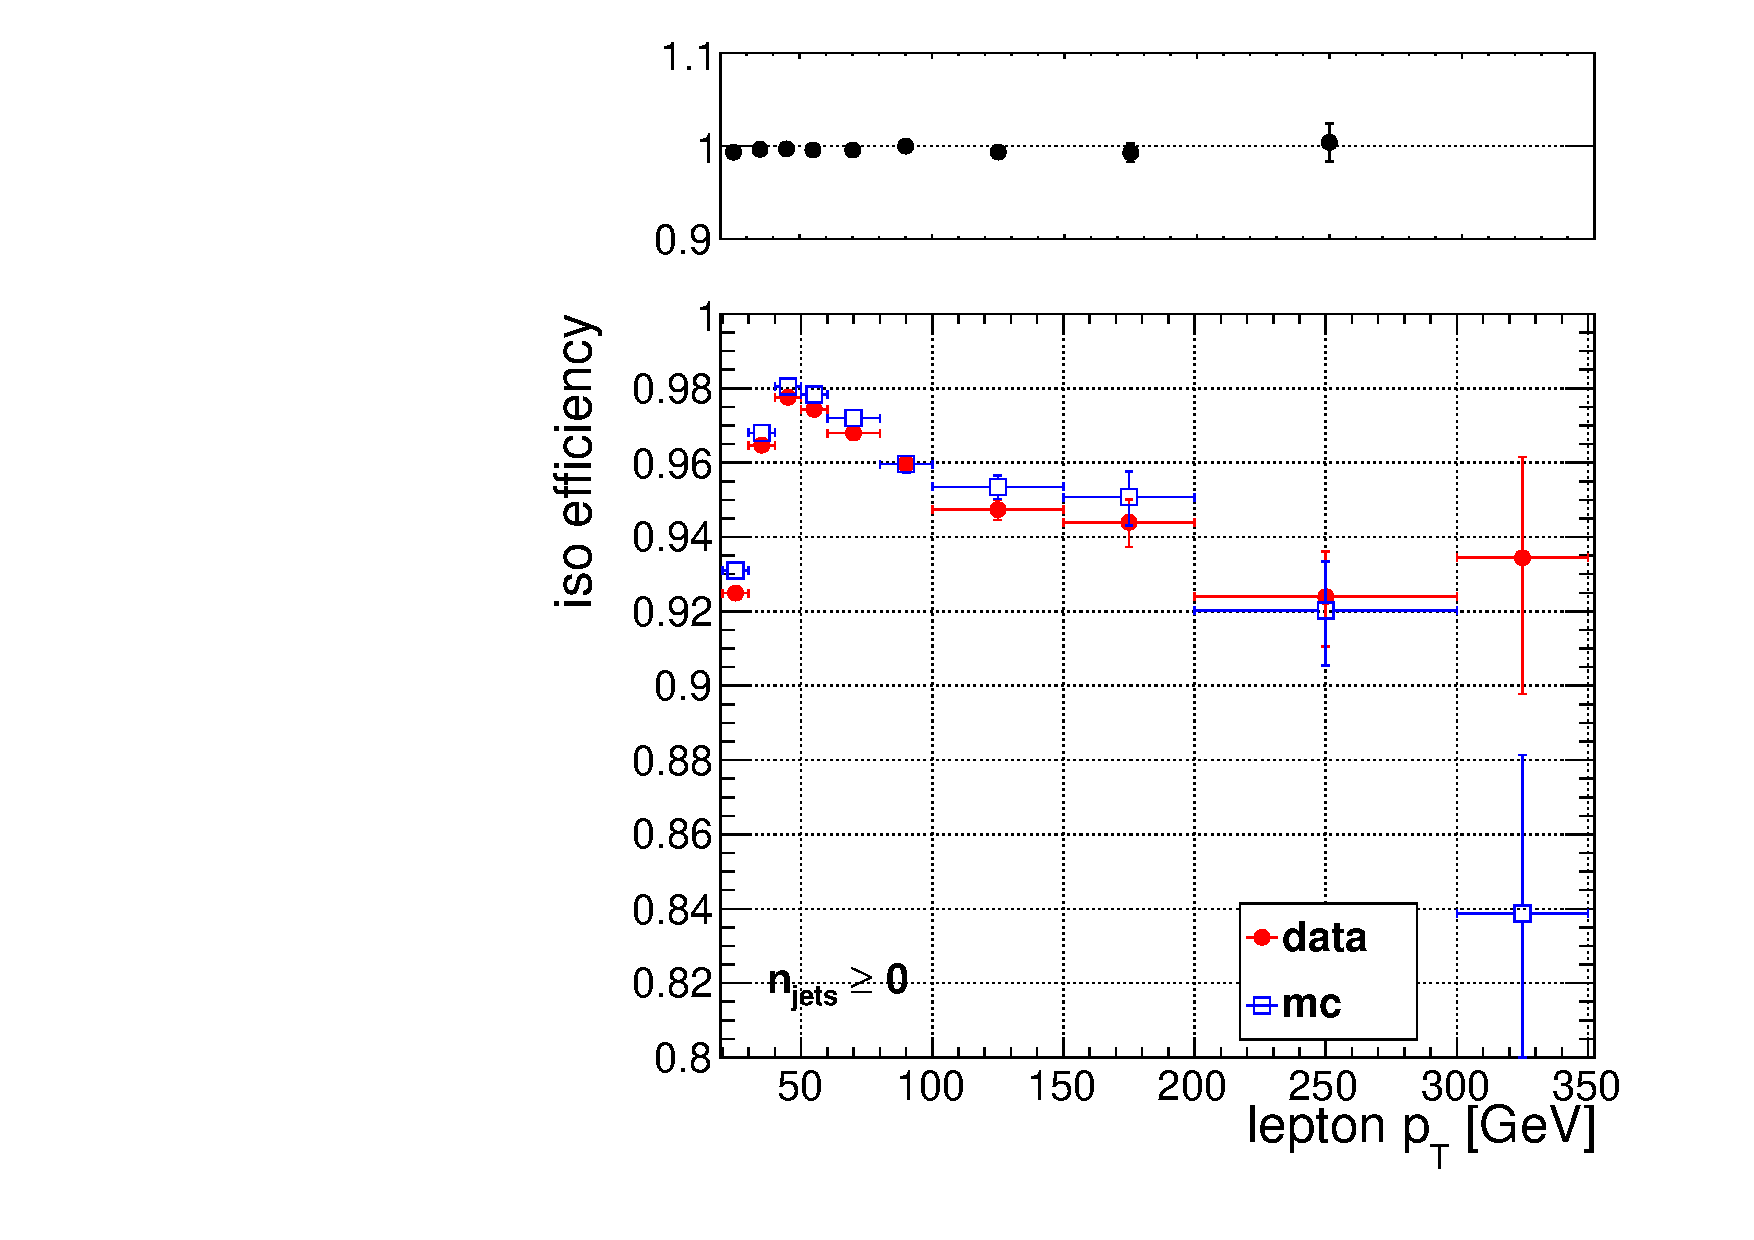
\includegraphics[width=0.3\linewidth]{plots/el_iso_njets0.pdf}
	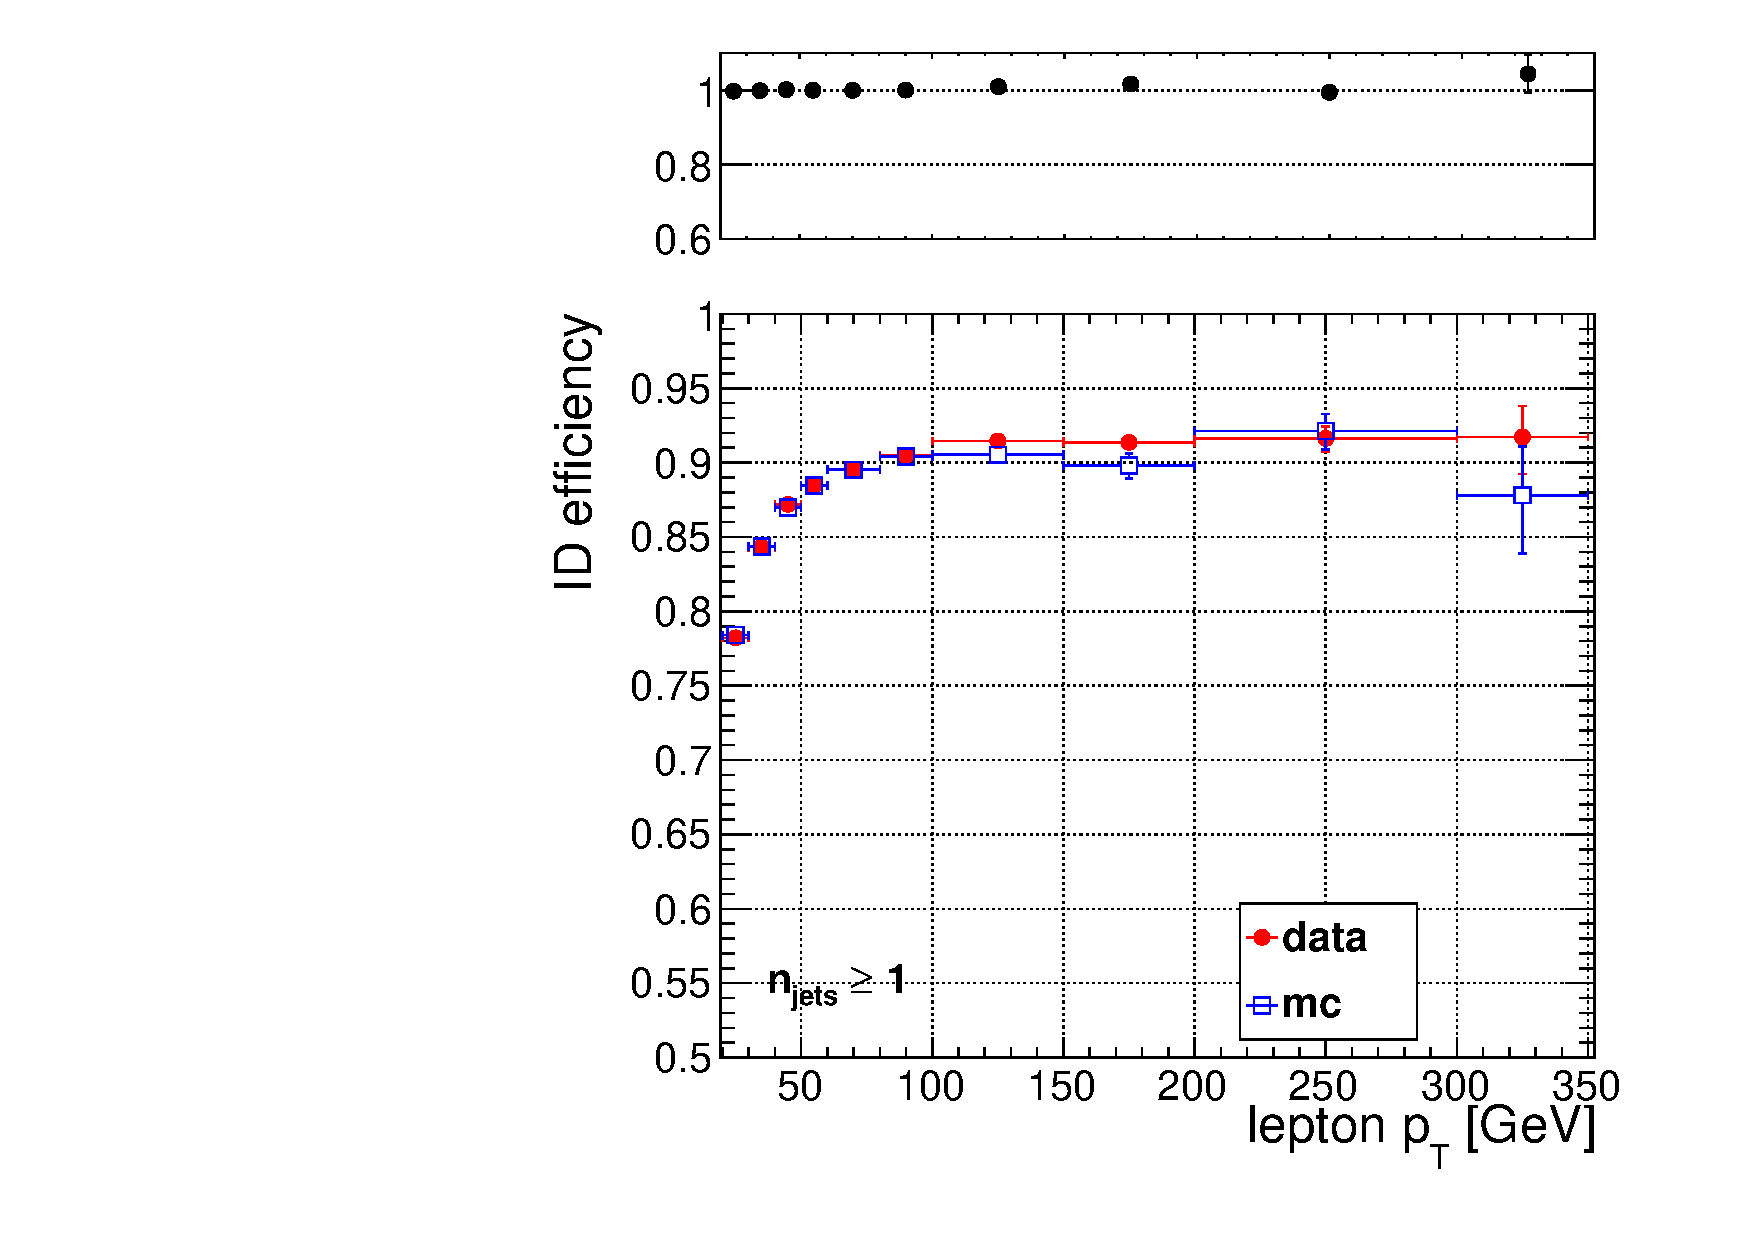
\includegraphics[width=0.3\linewidth]{plots/el_id_njets1.pdf}%
	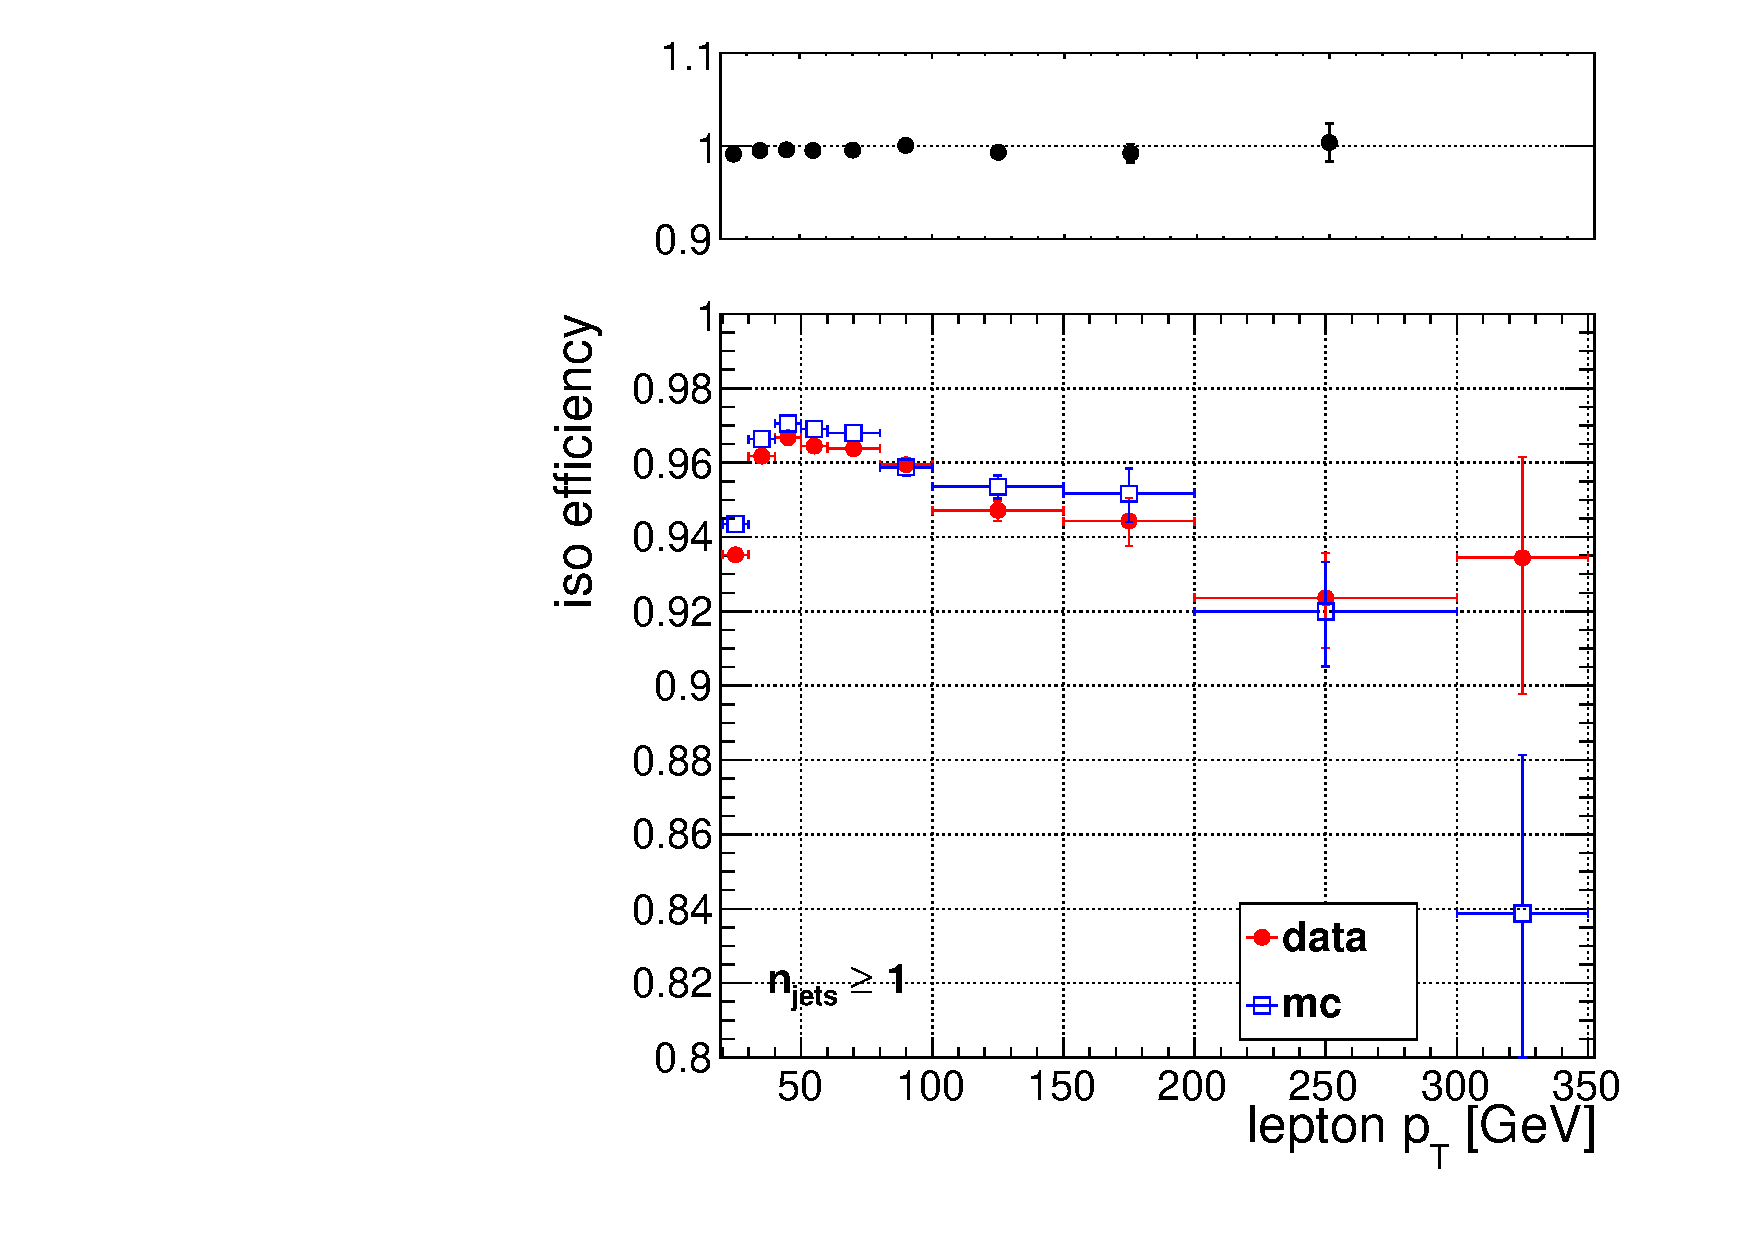
\includegraphics[width=0.3\linewidth]{plots/el_iso_njets1.pdf}
	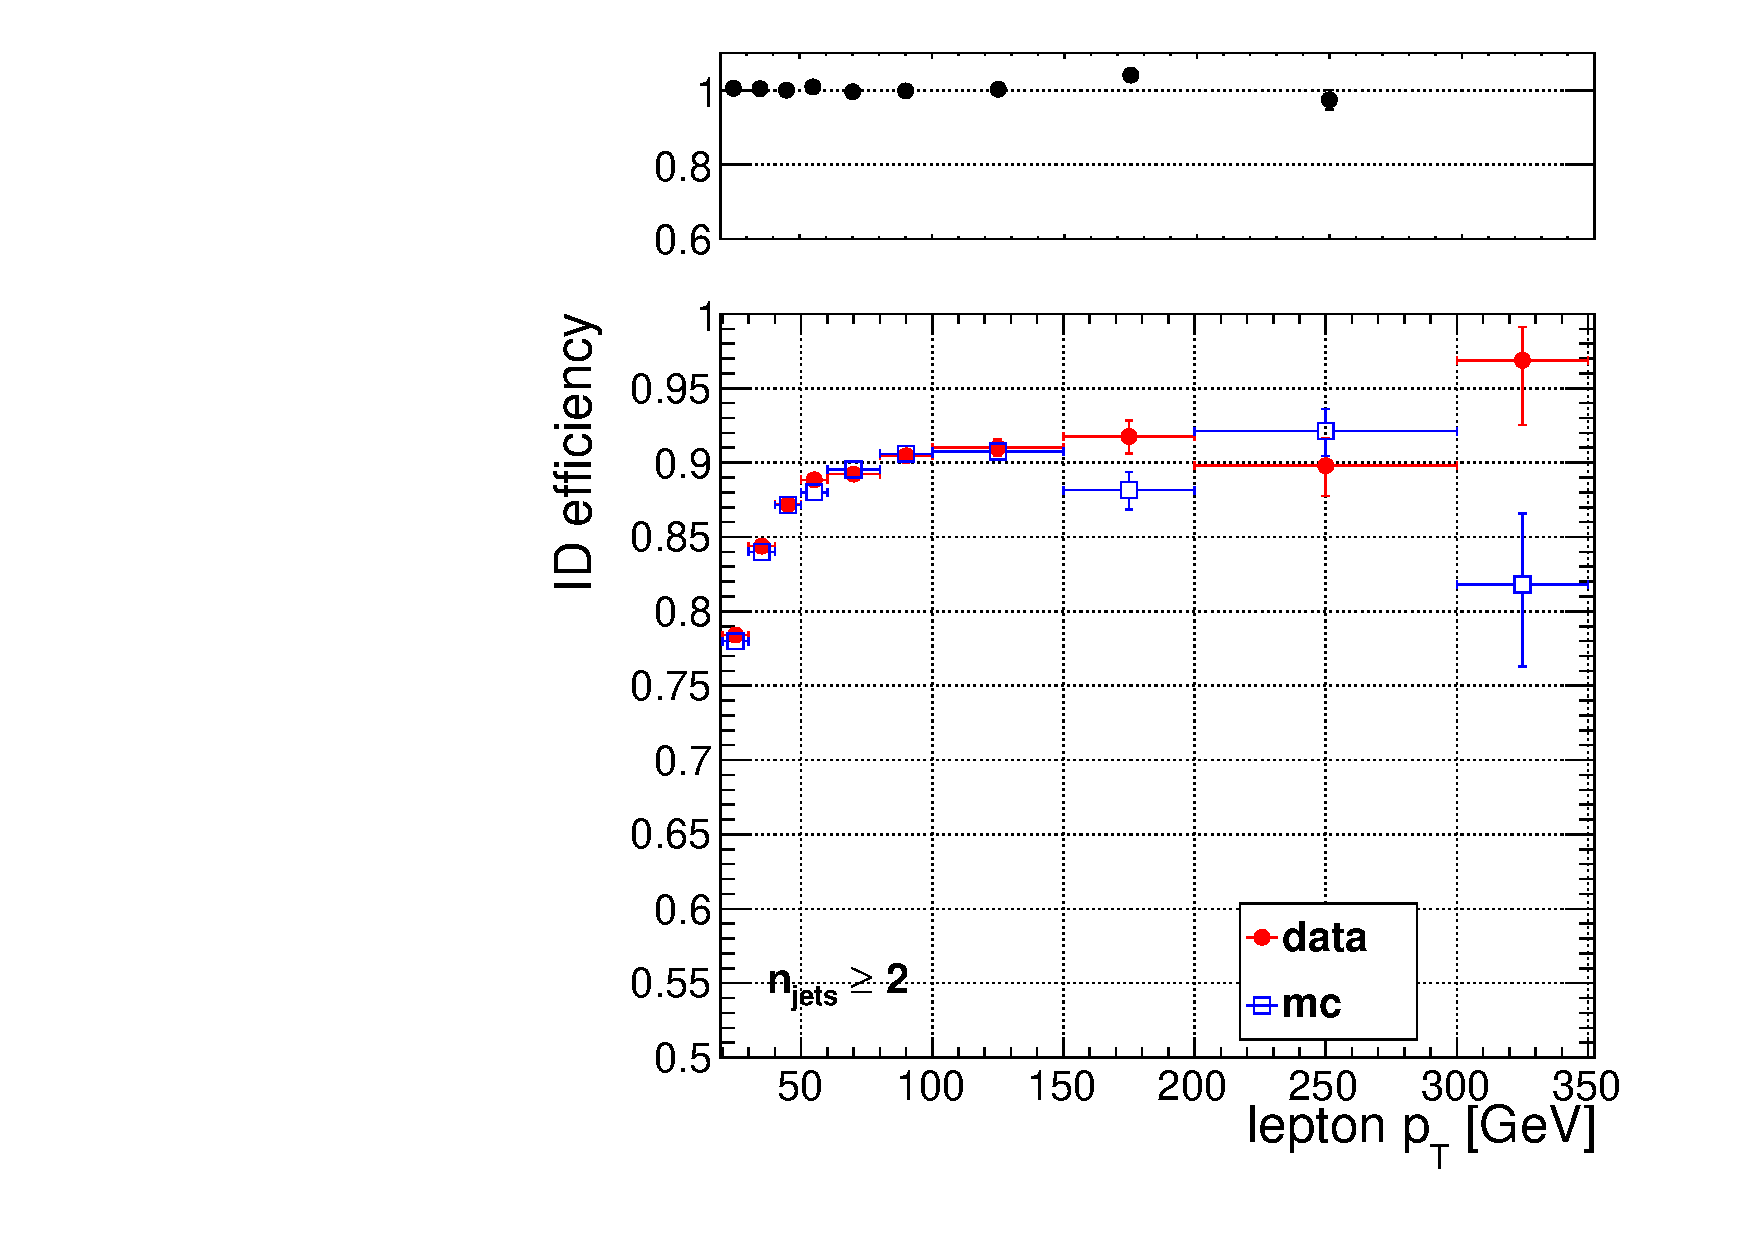
\includegraphics[width=0.3\linewidth]{plots/el_id_njets2.pdf}%
	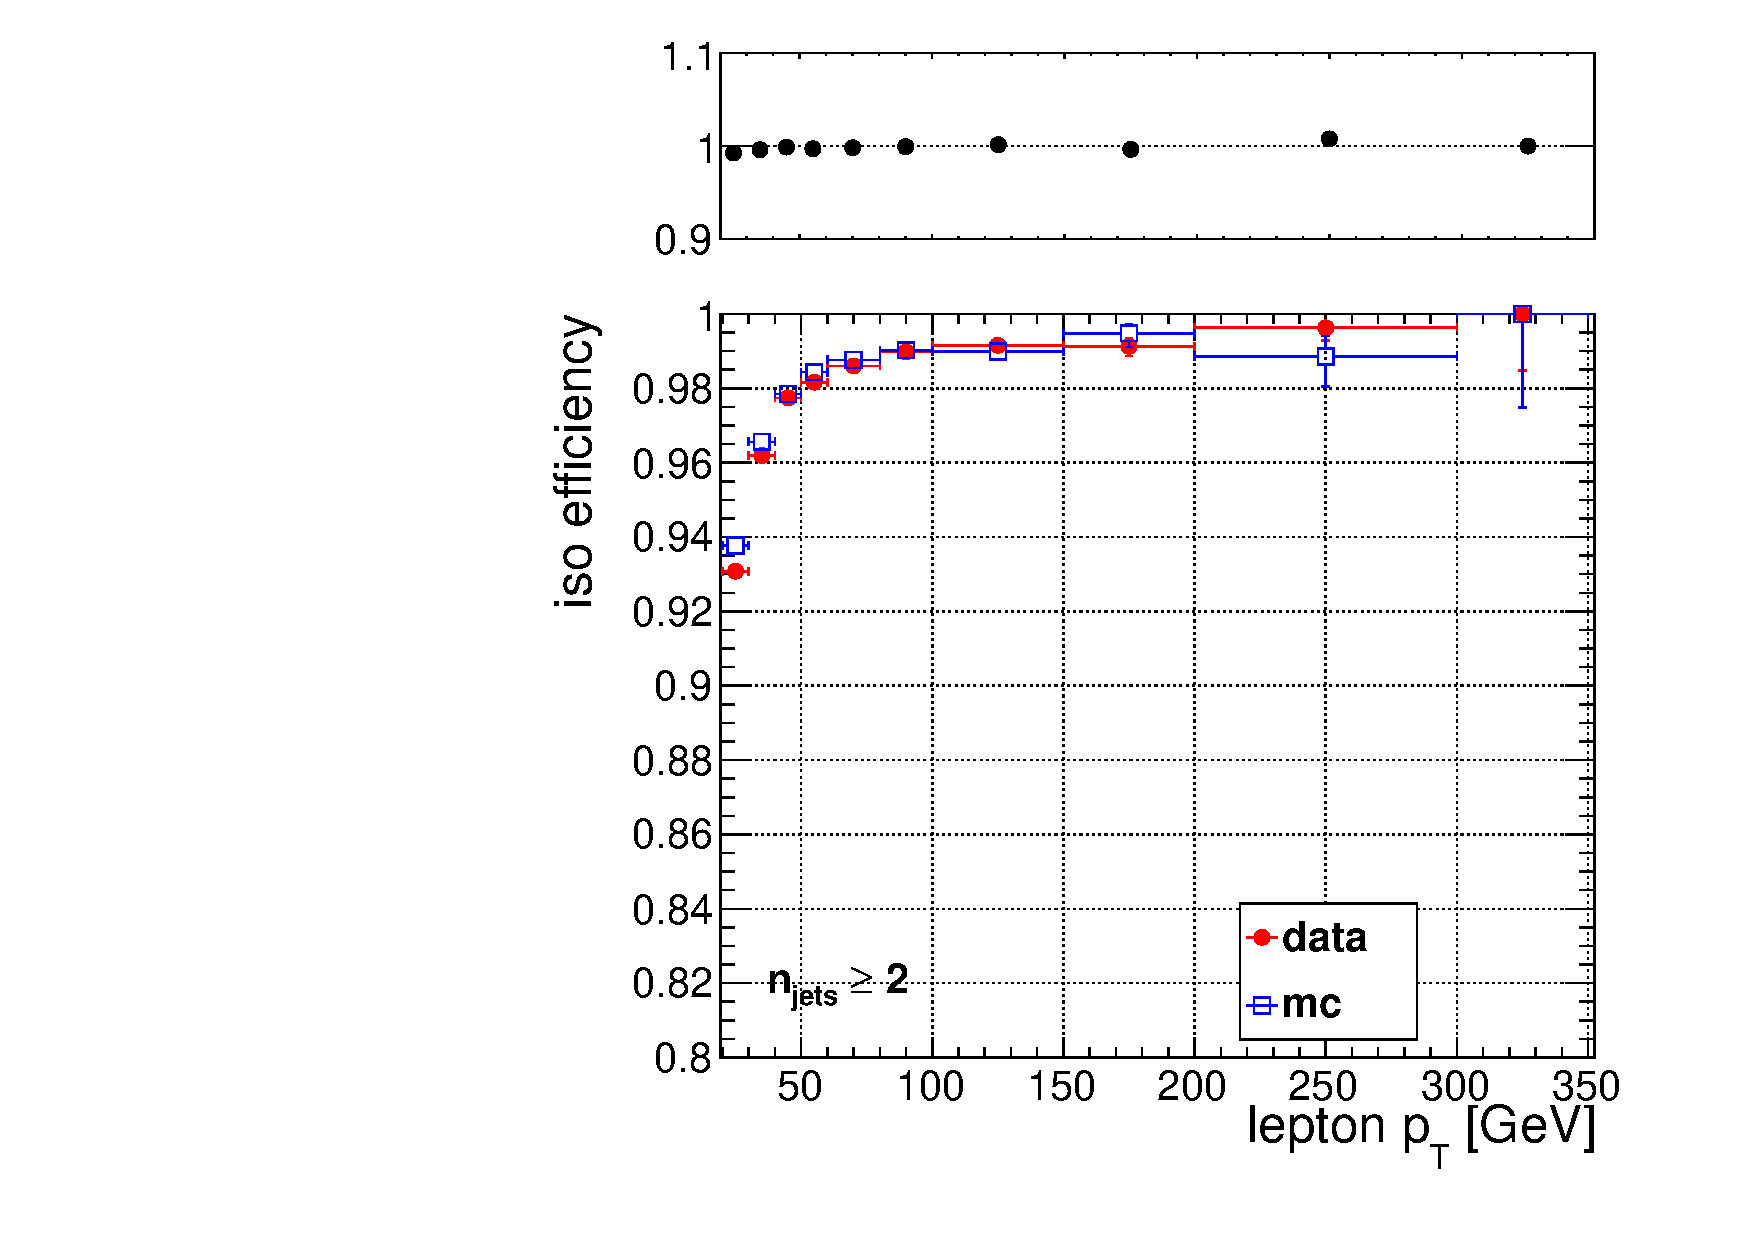
\includegraphics[width=0.3\linewidth]{plots/el_iso_njets2.pdf}
	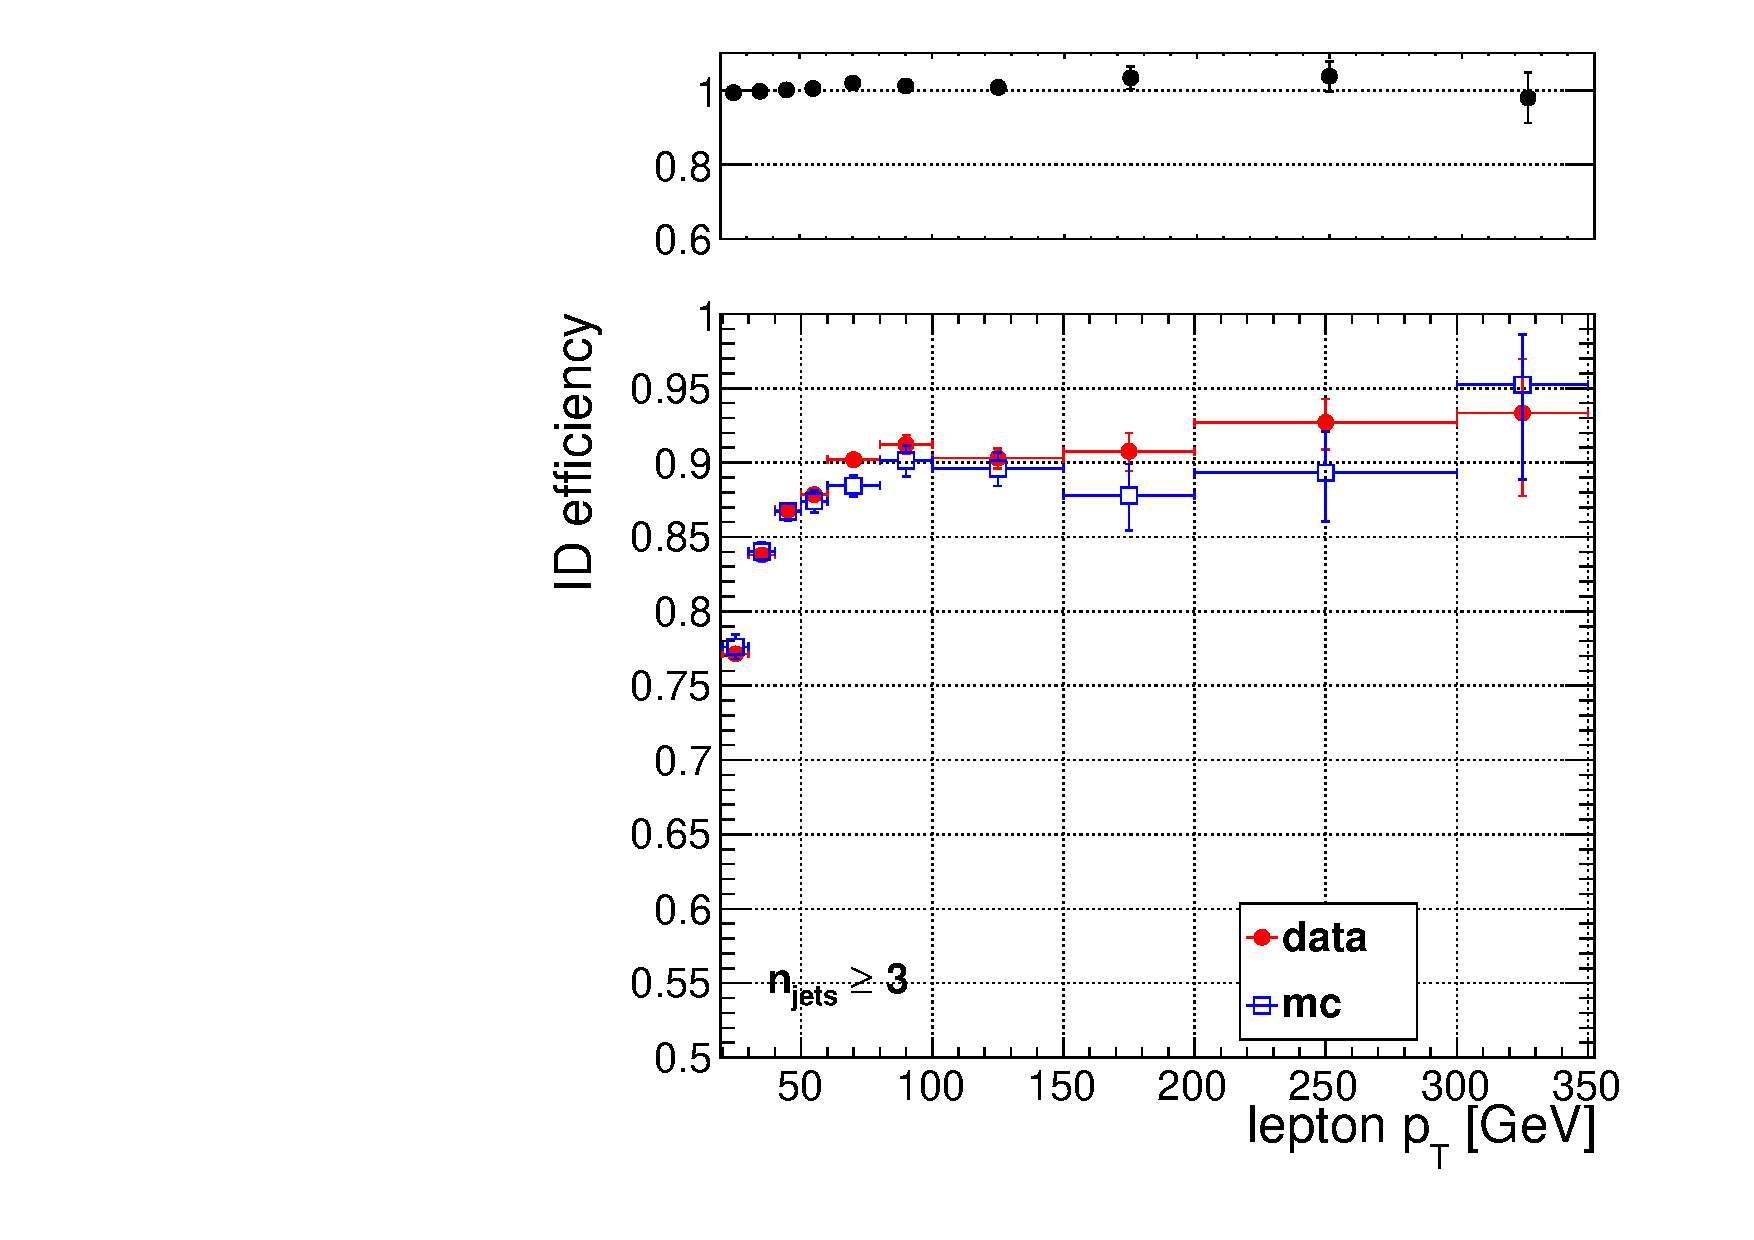
\includegraphics[width=0.3\linewidth]{plots/el_id_njets3.pdf}%
	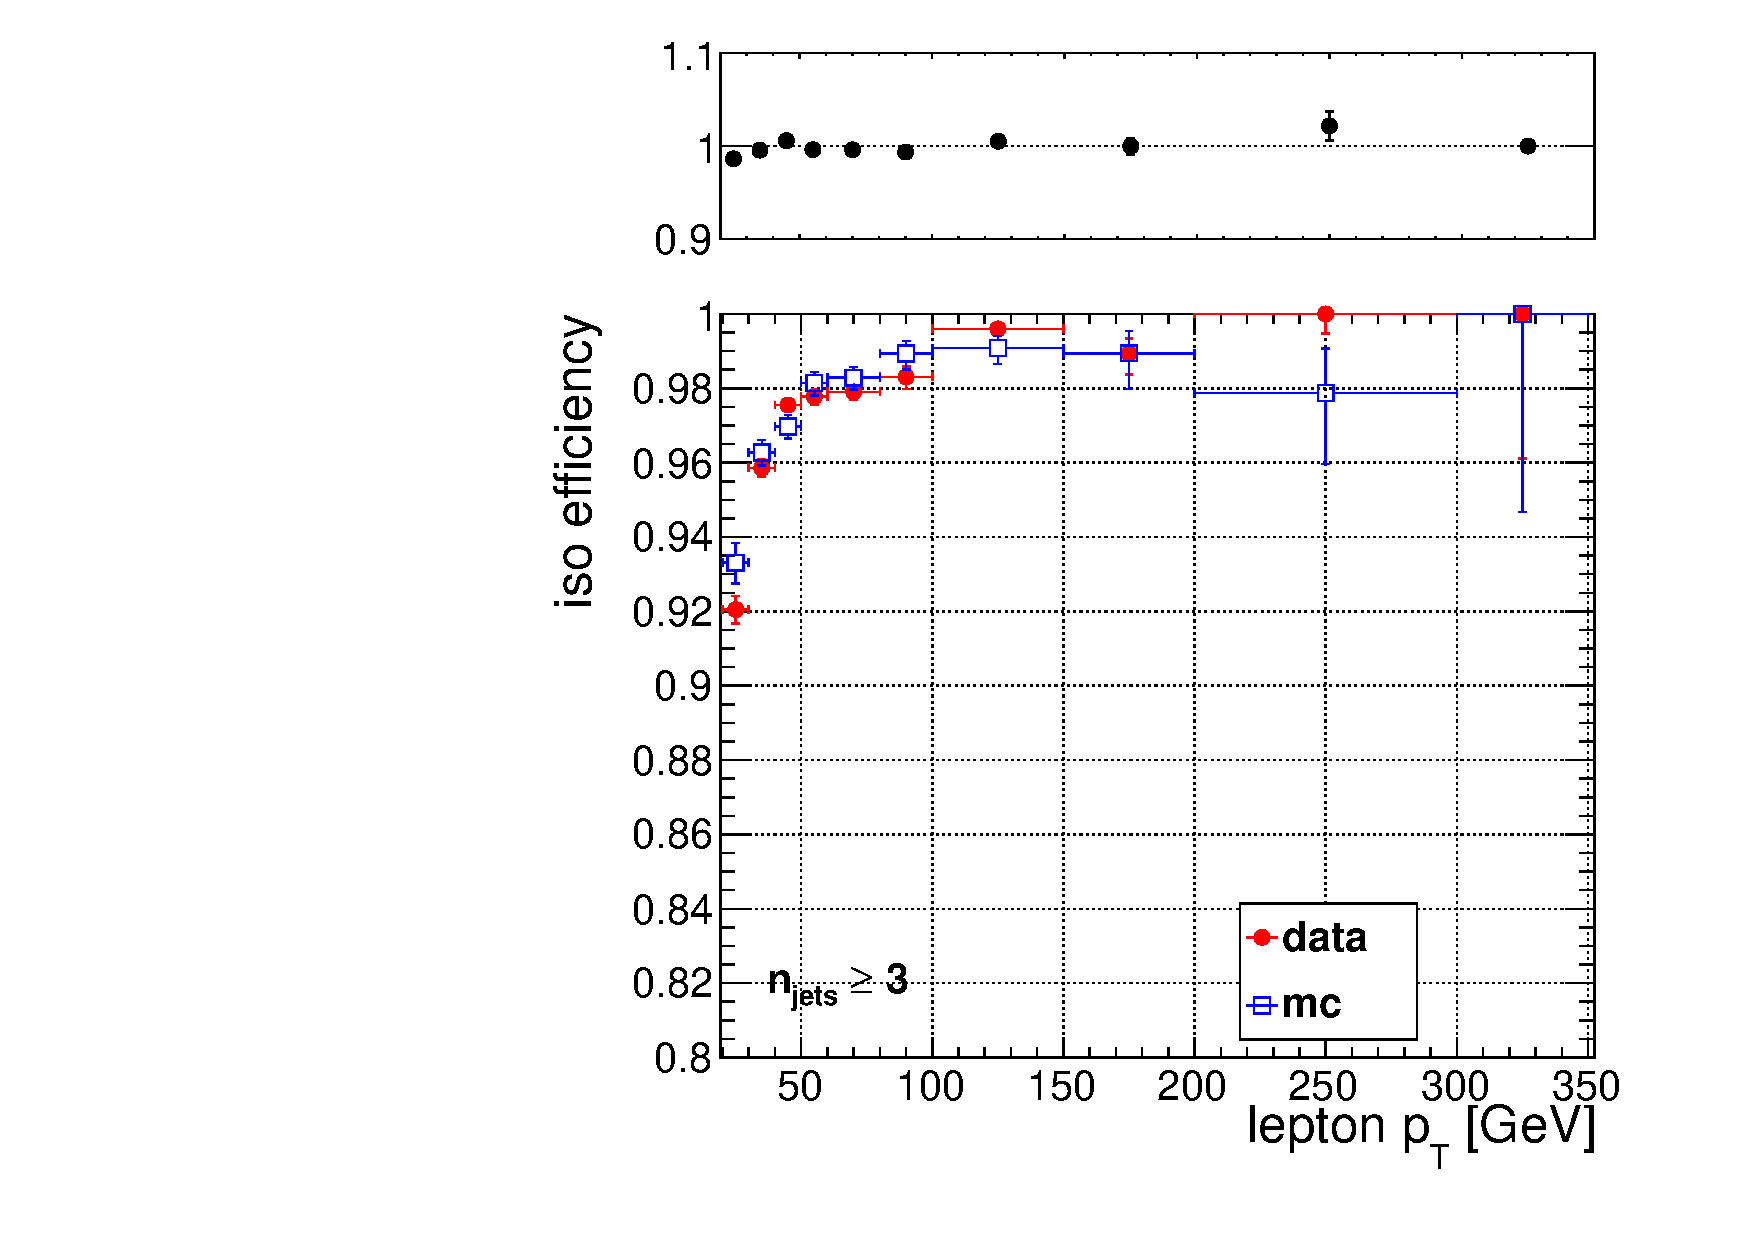
\includegraphics[width=0.3\linewidth]{plots/el_iso_njets3.pdf}
	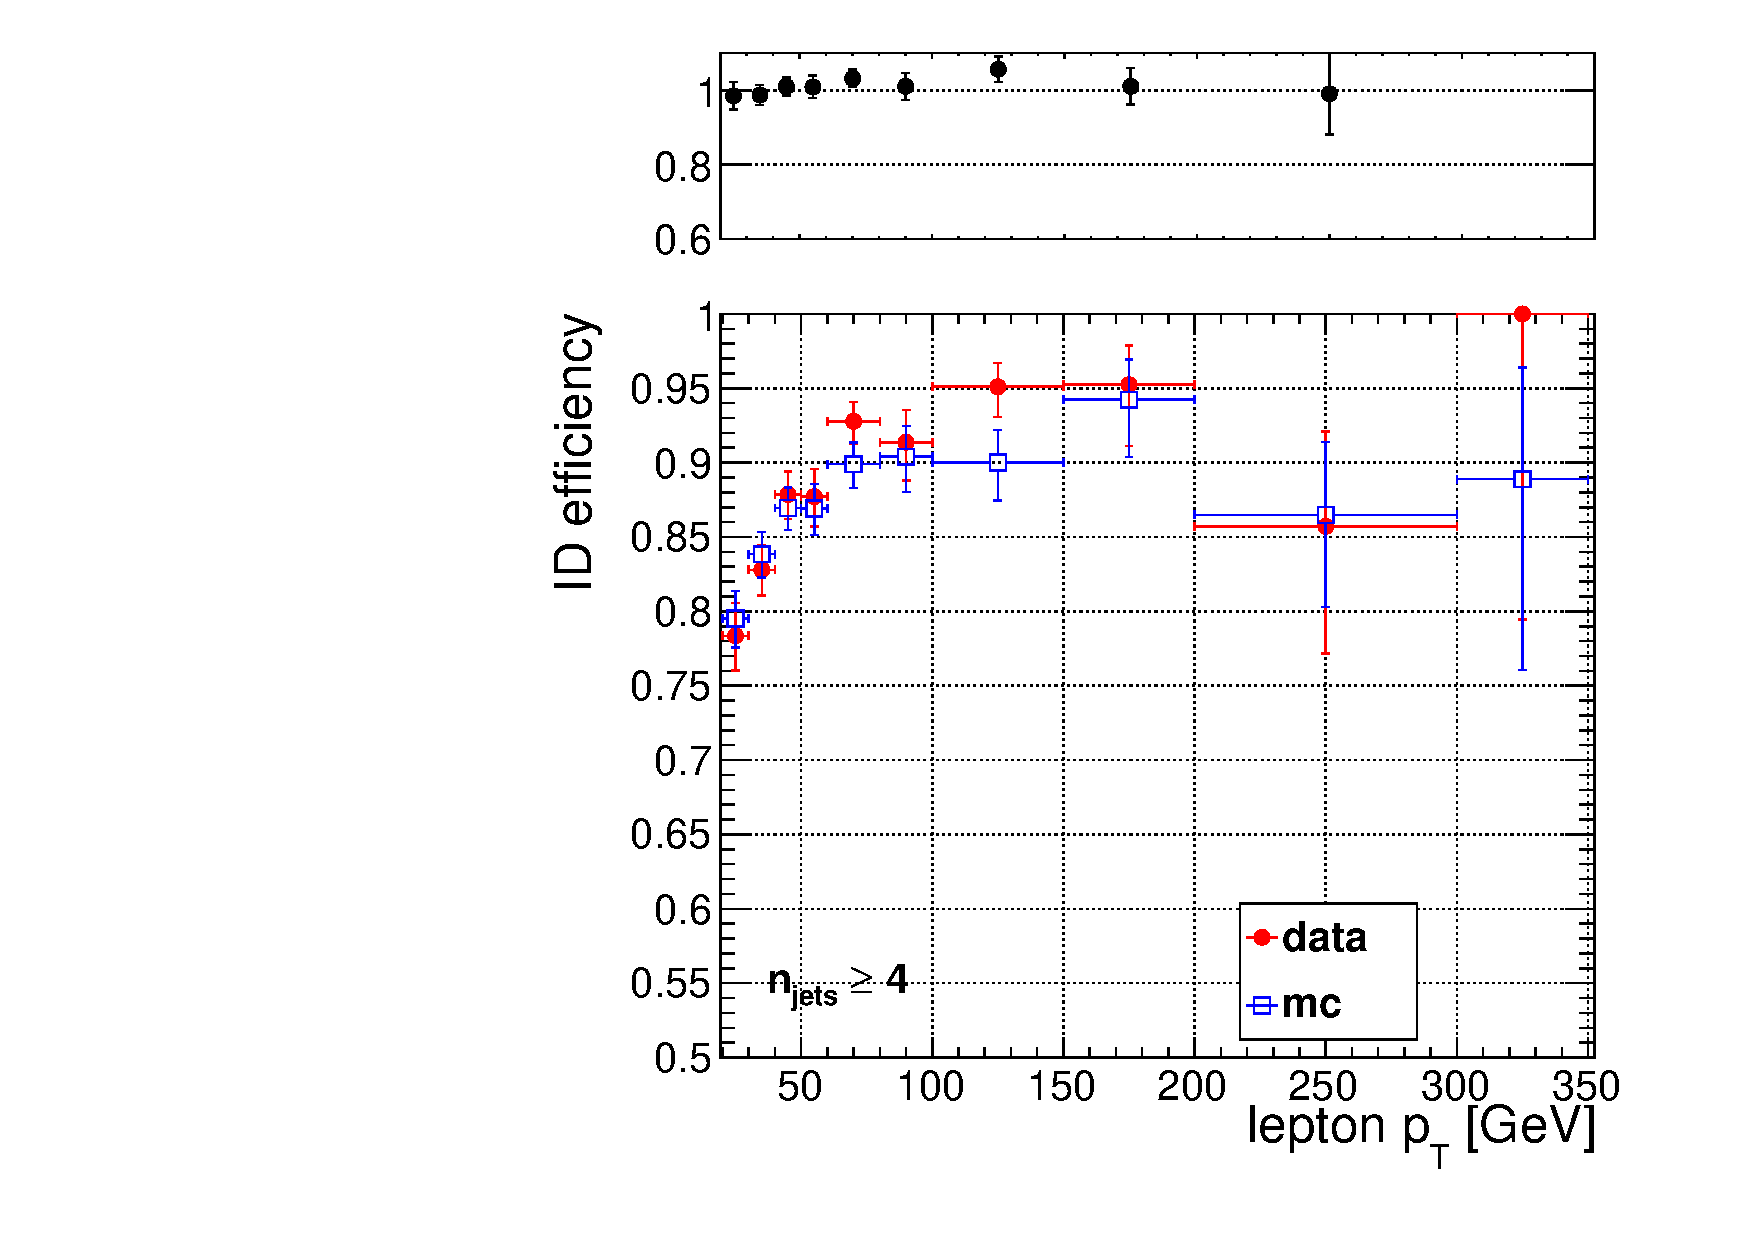
\includegraphics[width=0.3\linewidth]{plots/el_id_njets4.pdf}%
	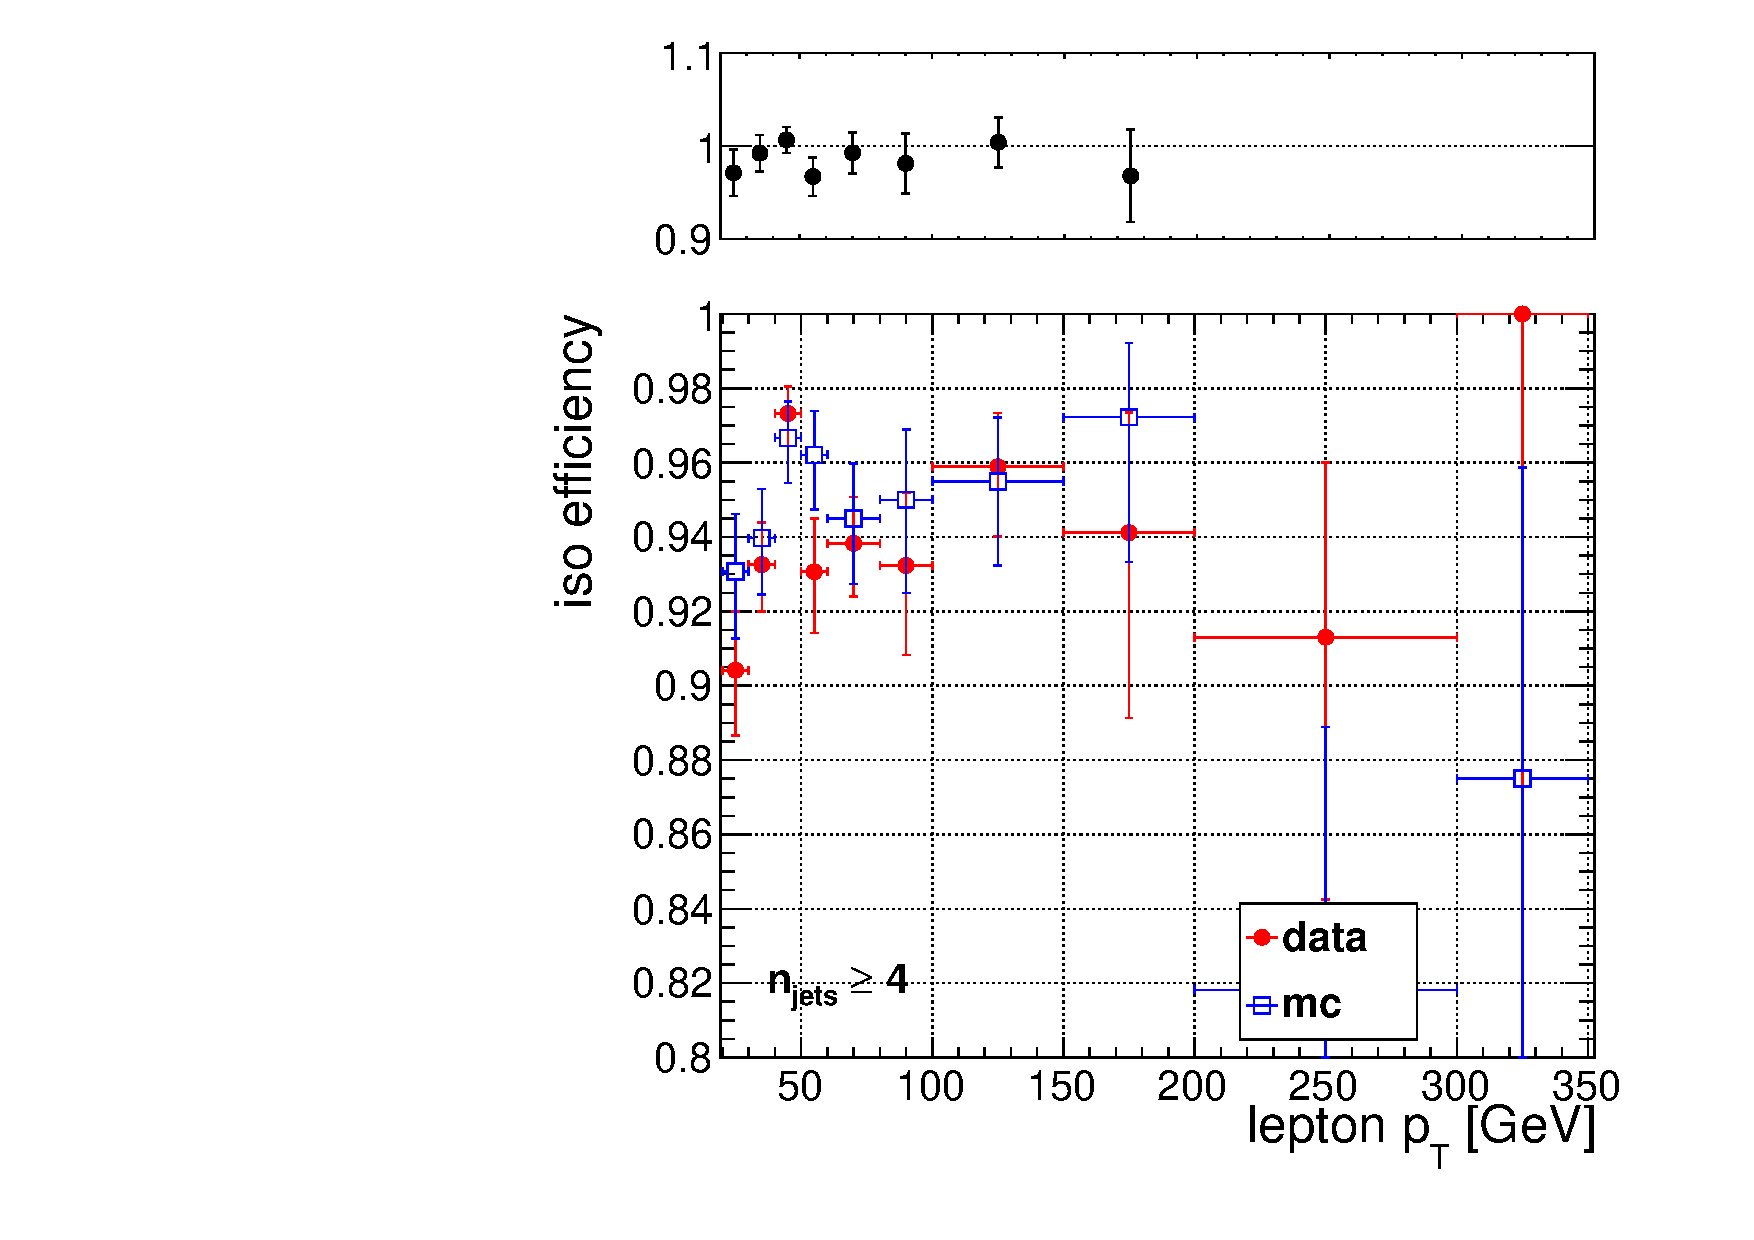
\includegraphics[width=0.3\linewidth]{plots/el_iso_njets4.pdf}
	\caption{
	  \label{fig:eltnpeff} Comparison of the electron identification and isolation efficiencies in data and MC for various jet multiplicity requirements. }  
      \end{center}
\end{figure}

\clearpage


\subsection{Trigger Efficiency Measurements}
\label{sec:trg}

In this section we measure the efficiencies of the single lepton triggers, HLT\_IsoMu24(\_eta2p1) for muons and HLT\_Ele27\_WP80 for electrons, using a tag-and-probe
approach. The tag is required to pass the full offline analysis selection and have \pt\ $>$ 30 GeV, $|\eta|<2.1$, and be matched to the single
lepton trigger. The probe is also required to pass the full offline analysis selection and have $|\eta|<2.1$, but the \pt\ requirement is relaxed to 20 GeV
in order to measure the \pt\ turn-on curve. The tag-probe pair is
required to have opposite-sign and an invariant mass in the range
76--106 GeV.

The measured trigger efficiencies are displayed in Fig.~\ref{fig:trigeff} and summarized in Table~\ref{tab:mutriggeff} (muons) and Table~\ref{tab:eltriggeff} (electrons).
These trigger efficiencies are applied to the MC when used to predict data yields selected by single lepton triggers.


\begin{figure}[!ht]
\begin{center}
\begin{tabular}{cc}
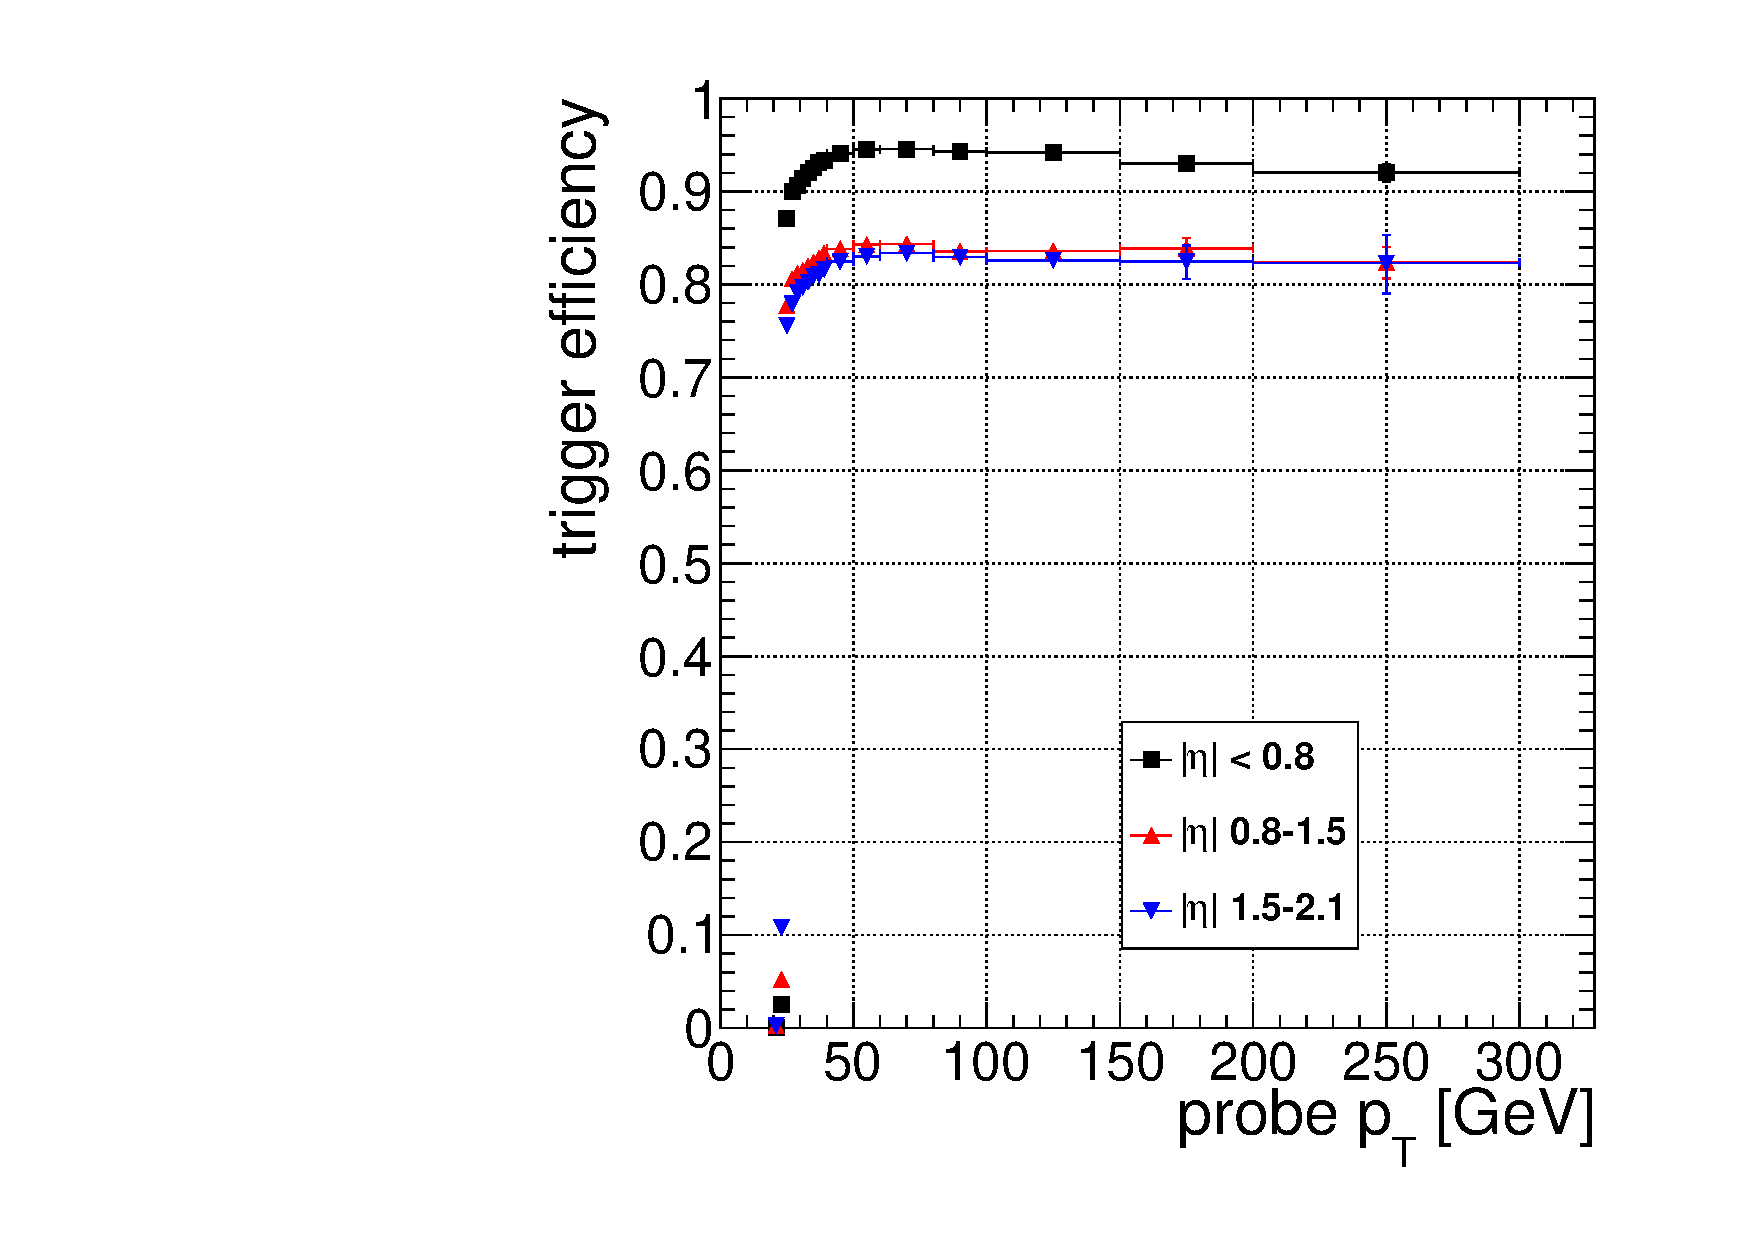
\includegraphics[width=0.4\textwidth]{plots/mutrig_pt_etabins.pdf} &
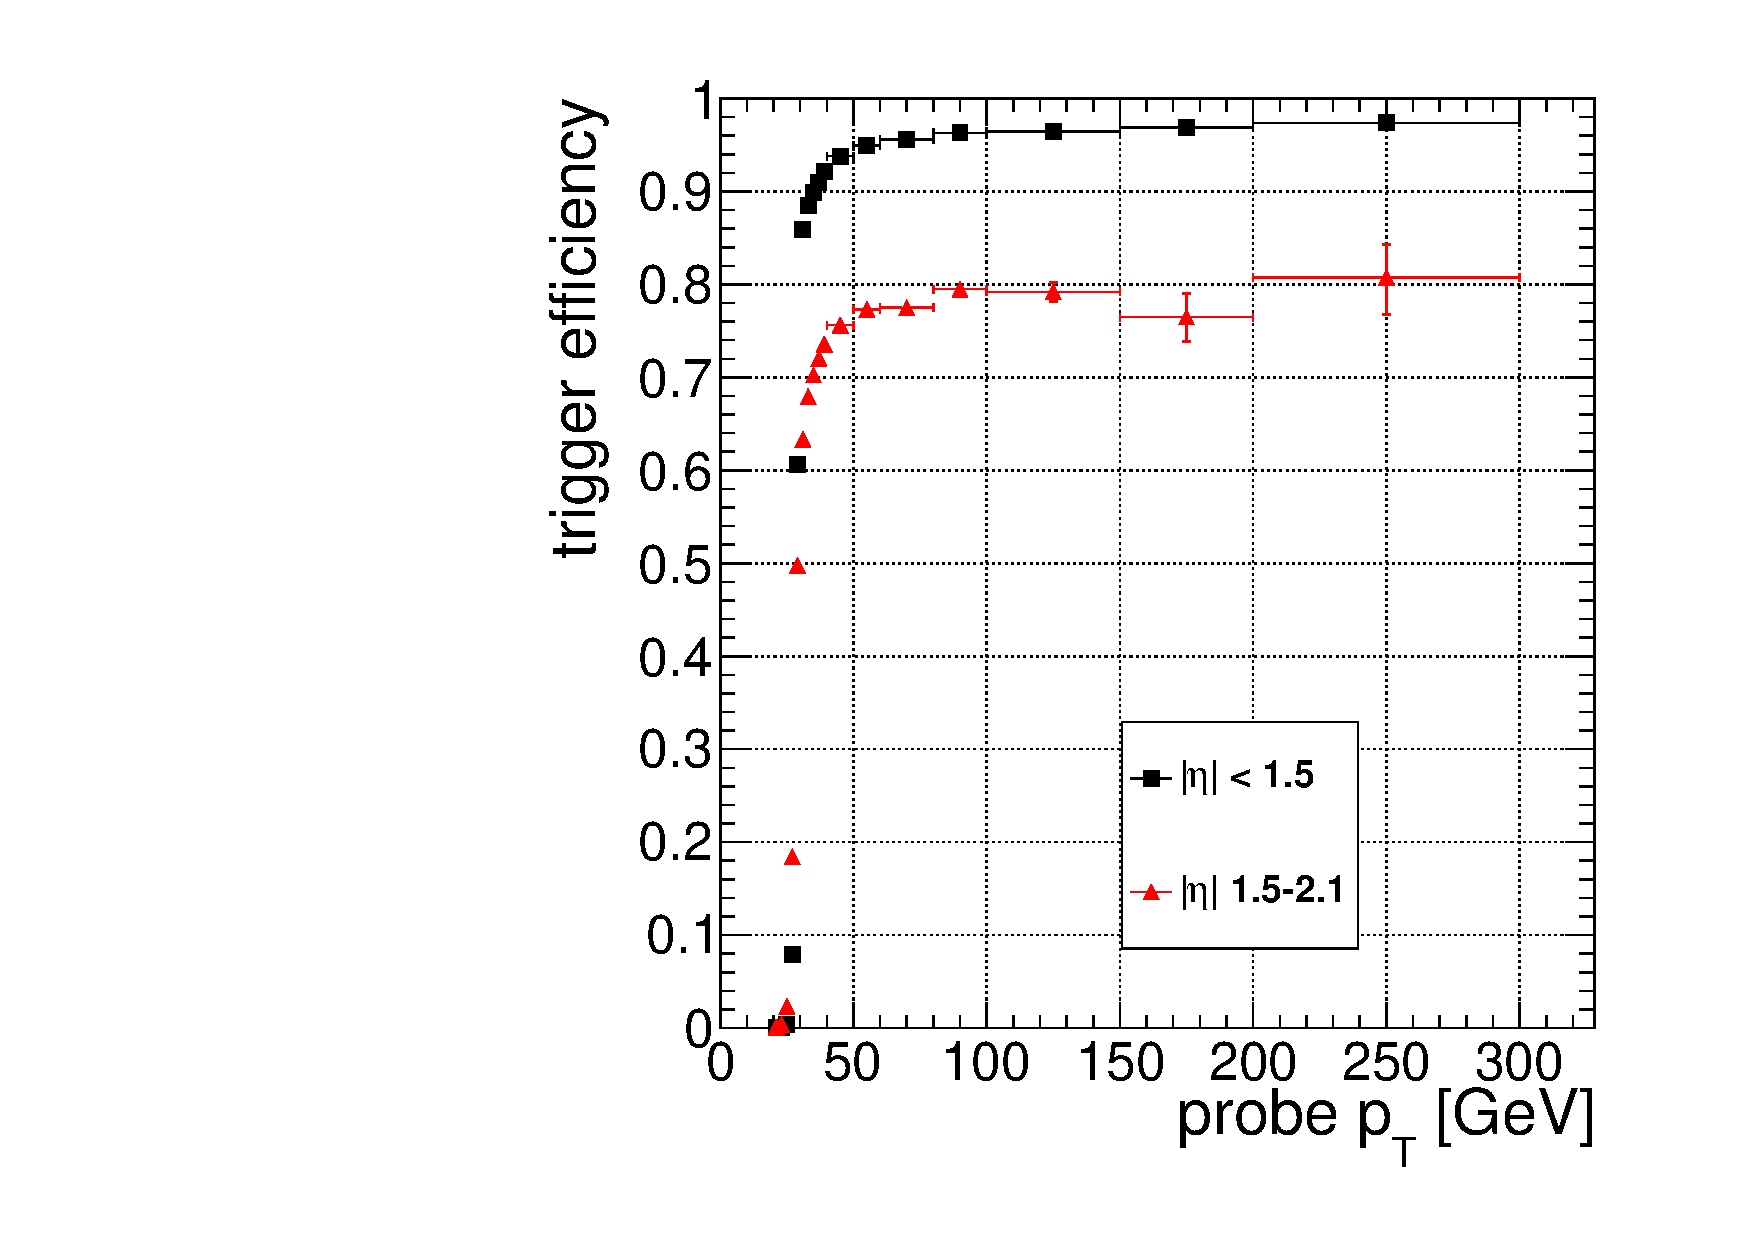
\includegraphics[width=0.4\textwidth]{plots/eltrig_pt_etabins.pdf} \\
\end{tabular}
\caption{\label{fig:trigeff}
Efficiency for the single muon trigger HLT\_IsoMu24(\_eta2p1) (left) and single electron trigger HLT\_Ele27\_WP80 (right) as a function of lepton \pt,
for several bins in lepton $|\eta|$.
}
\end{center}
\end{figure}

\clearpage

\begin{table}[htb]
\begin{center}
\footnotesize
\caption{\label{tab:mutriggeff}
Summary of the single muon trigger efficiency HLT\_IsoMu24(\_eta2p1). Uncertainties are statistical.}
\begin{tabular}{c|c|c|c}

% Selection            : (((((((((abs(tagAndProbeMass-91)<15)&&(qProbe*qTag<0))&&((eventSelection&2)==2))&&(HLT_IsoMu24_tag > 0))&&(tag->pt()>30.0))&&(abs(tag->eta())<2.1))&&(probe->pt()>20))&&(abs(probe->eta())<2.1))&&((leptonSelection&65536)==65536))&&((leptonSelection&131072)==131072)
% Probe trigger        : HLT_IsoMu24_probe > 0
% Total data yield     : 5161723

\hline
\hline
  \pt\ range [GeV] & $|\eta|<0.8$ & $0.8<|\eta|<1.5$ & $1.5<|\eta|<2.1$ \\
\hline
  20 -  22  & 	0.00 $\pm$ 0.000 & 	0.00 $\pm$ 0.000 & 	0.00 $\pm$ 0.000 \\
  22 -  24  & 	0.03 $\pm$ 0.001 & 	0.05 $\pm$ 0.001 & 	0.11 $\pm$ 0.002 \\
  24 -  26  & 	0.87 $\pm$ 0.002 & 	0.78 $\pm$ 0.002 & 	0.76 $\pm$ 0.003 \\
  26 -  28  & 	0.90 $\pm$ 0.001 & 	0.81 $\pm$ 0.002 & 	0.78 $\pm$ 0.002 \\
  28 -  30  & 	0.91 $\pm$ 0.001 & 	0.81 $\pm$ 0.002 & 	0.79 $\pm$ 0.002 \\
  30 -  32  & 	0.91 $\pm$ 0.001 & 	0.81 $\pm$ 0.001 & 	0.80 $\pm$ 0.002 \\
  32 -  34  & 	0.92 $\pm$ 0.001 & 	0.82 $\pm$ 0.001 & 	0.80 $\pm$ 0.002 \\
  34 -  36  & 	0.93 $\pm$ 0.001 & 	0.82 $\pm$ 0.001 & 	0.81 $\pm$ 0.001 \\
  36 -  38  & 	0.93 $\pm$ 0.001 & 	0.83 $\pm$ 0.001 & 	0.81 $\pm$ 0.001 \\
  38 -  40  & 	0.93 $\pm$ 0.001 & 	0.83 $\pm$ 0.001 & 	0.82 $\pm$ 0.001 \\
  40 -  50  & 	0.94 $\pm$ 0.000 & 	0.84 $\pm$ 0.000 & 	0.82 $\pm$ 0.001 \\
  50 -  60  & 	0.95 $\pm$ 0.000 & 	0.84 $\pm$ 0.001 & 	0.83 $\pm$ 0.001 \\
  60 -  80  & 	0.95 $\pm$ 0.001 & 	0.84 $\pm$ 0.002 & 	0.83 $\pm$ 0.002 \\
  80 - 100  & 	0.94 $\pm$ 0.002 & 	0.84 $\pm$ 0.004 & 	0.83 $\pm$ 0.006 \\
 100 - 150  & 	0.94 $\pm$ 0.003 & 	0.84 $\pm$ 0.005 & 	0.83 $\pm$ 0.008 \\
 150 - 200  & 	0.93 $\pm$ 0.006 & 	0.84 $\pm$ 0.011 & 	0.82 $\pm$ 0.018 \\
 $>$200     & 	0.92 $\pm$ 0.010 & 	0.82 $\pm$ 0.017 & 	0.82 $\pm$ 0.031 \\
\hline
\hline

\end{tabular}
\end{center}
\end{table}

\begin{table}[htb]
\begin{center}
\footnotesize
\caption{\label{tab:eltriggeff}
Summary of the single electron trigger efficiency HLT\_Ele27\_WP80. Uncertainties are statistical.}
\begin{tabular}{c|c|c}

% Selection            : (((((((((abs(tagAndProbeMass-91)<15)&&(qProbe*qTag<0))&&((eventSelection&1)==1))&&(HLT_Ele27_WP80_tag > 0))&&(tag->pt()>30.0))&&(abs(tag->eta())<2.1))&&(probe->pt()>20))&&(abs(probe->eta())<2.1))&&((leptonSelection&8)==8))&&((leptonSelection&16)==16)
% Probe trigger        : HLT_Ele27_WP80_probe > 0
% Total data yield     : 3405966

\hline
\hline
  \pt\ range [GeV] & $|\eta|<1.5$ & $1.5<|\eta|<2.1$ \\
\hline
  20 -  22   & 	0.00 $\pm$ 0.000 & 	0.00 $\pm$ 0.000 \\
  22 -  24   & 	0.00 $\pm$ 0.000 & 	0.00 $\pm$ 0.001 \\
  24 -  26   & 	0.00 $\pm$ 0.000 & 	0.02 $\pm$ 0.001 \\
  26 -  28   & 	0.08 $\pm$ 0.001 & 	0.18 $\pm$ 0.003 \\
  28 -  30   & 	0.61 $\pm$ 0.002 & 	0.50 $\pm$ 0.004 \\
  30 -  32   & 	0.86 $\pm$ 0.001 & 	0.63 $\pm$ 0.003 \\
  32 -  34   & 	0.88 $\pm$ 0.001 & 	0.68 $\pm$ 0.003 \\
  34 -  36   & 	0.90 $\pm$ 0.001 & 	0.70 $\pm$ 0.002 \\
  36 -  38   & 	0.91 $\pm$ 0.001 & 	0.72 $\pm$ 0.002 \\
  38 -  40   & 	0.92 $\pm$ 0.001 & 	0.74 $\pm$ 0.002 \\
  40 -  50   & 	0.94 $\pm$ 0.000 & 	0.76 $\pm$ 0.001 \\
  50 -  60   & 	0.95 $\pm$ 0.000 & 	0.77 $\pm$ 0.002 \\
  60 -  80   & 	0.96 $\pm$ 0.001 & 	0.78 $\pm$ 0.003 \\
  80 - 100   & 	0.96 $\pm$ 0.002 & 	0.80 $\pm$ 0.008 \\
  100 - 150  & 	0.96 $\pm$ 0.002 & 	0.79 $\pm$ 0.010 \\
  150 - 200  & 	0.97 $\pm$ 0.004 & 	0.76 $\pm$ 0.026 \\
$>$200       & 	0.97 $\pm$ 0.005 & 	0.81 $\pm$ 0.038 \\
\hline
\hline

\end{tabular}
\end{center}
\end{table}

\clearpage
